\documentclass[11pt]{article}
\usepackage[margin=24mm]{geometry}
\usepackage{amsmath,amssymb,amsthm,mathtools,bm,graphicx,booktabs,microtype}
\usepackage[numbers,sort&compress]{natbib}
\usepackage[colorlinks=true,allcolors=blue]{hyperref}
\usepackage[font=small,labelfont=bf]{caption}
\usepackage{placeins}
\renewcommand{\topfraction}{.95}
\renewcommand{\bottomfraction}{.85}
\renewcommand{\textfraction}{.05}
\renewcommand{\floatpagefraction}{.65}
\setcounter{topnumber}{3}
\setcounter{bottomnumber}{2}
\clubpenalty=10000
\widowpenalty=10000
\displaywidowpenalty=10000
\newcommand{\E}{\mathbb E}
\newcommand{\dd}{\,\mathrm d}
\newcommand{\diag}{\operatorname{diag}}
\newcommand{\tr}{\operatorname{tr}}
\newcommand{\PR}{D}
\newcommand{\energy}{\mathcal E}
\newtheorem{proposition}{Proposition}
\graphicspath{{figures/}{../experiments/figures/}{../experiments/degree/}{../archive/research_round/record/}}
\hypersetup{pdftitle={Conditional activity geometry in balanced excitatory-inhibitory networks}}
\title{Conditional activity geometry in balanced\\excitatory--inhibitory networks}
\author{}
\date{Working manuscript, 19 November 2026}
\begin{document}
\maketitle
\begin{abstract}
Excitation--inhibition balance creates heterogeneous neuronal operating points
even when neurons share a transfer function. These operating points jointly
determine temporal variances and local responses, so replacing the population
by an average neuron can distort its collective activity geometry. We combine
conditional balanced-network mean field with a two-site cavity closure to
obtain a population resolvent for E--E, E--I, and I--I covariance energies and
the participation ratio, including normalized temporal alignment between the
populations. Under stated common-leak stability assumptions,
averaging conditional spectra or gains before taking their second moments
raises the predicted dimension, with a blockwise inequality for covariance
energy. The calculation separates two interventions: changing population
fractions at fixed aggregate coupling reweights geometry, whereas changing
degree dispersion alters the self-consistent operating-point distribution.
Strict Dale-network comparisons reproduce a large degree-driven change in
dimension and expose quantitative finite-network deviations, alongside the
importance of finite-record centering. The resulting conditional prediction
of activity geometry separates its algebraic consequences from its empirical
accuracy; it does not supply a full finite-network covariance spectrum or a
theorem of nonlinear cavity decoupling.
\end{abstract}

\section{From balanced activity to collective dimension}

Large excitatory and inhibitory inputs can cancel in their mean while leaving
fluctuations comparable to the residual input. This balanced regime provides
a mechanism for irregular activity \citep{vreeswijk1996,kadmon2015}. It also
generates static differences between neurons: each incoming connectivity row
samples a different combination of presynaptic rates. A common microscopic
transfer function therefore need not imply a common distribution of activity
variance or response.

The question here is how those endogenous local differences shape covariance
geometry. Let $r_i(t)$ be a stationary rate trajectory, $m_i=\langle
r_i\rangle_t$, and
\begin{equation}
 C_{ij}(\tau)=\langle[r_i(t+\tau)-m_i][r_j(t)-m_j]\rangle_t.
 \label{eq:covariance}
\end{equation}
At zero lag, $C(0)$ is positive semidefinite. Its participation ratio is
\begin{equation}
 \PR=\frac{[\tr C(0)]^2}{\tr[C(0)^2]},\qquad
 \nu_N=\frac{\tr C(0)}{N},\quad
 \energy_N=\frac{\tr[C(0)^2]}{N},\quad
 d_N=\frac{\PR}{N}=\frac{\nu_N^2}{\energy_N}.
 \label{eq:pr}
\end{equation}
It measures how broadly variance is distributed among activity modes.
It is distinct from a Lyapunov dimension, and by itself does not establish
performance on a computational task.

Two-site cavity theory already predicts covariance energy and dimensionality
in random recurrent networks \citep{clark2023}. General neuronal heterogeneity,
including its different effects through recurrent gains and readout amplitudes,
is treated by \citet{clark2025}. Appendix J of that work already retains
same-label spectral and response products of the kind used below.
Balanced EI mean field supplies the
self-consistent distribution of local operating points, and earlier work
distinguishes fixed and fluctuating in-degree \citep{kadmon2015,mastrogiuseppe2017}.
Related cavity work for independent, identically distributed couplings derives
a linear-equivalent covariance description at fixed quenched connectivity
\citep{clark2026linear}. Here we target population
covariance energies and PR; an accurate covariance matrix for each individual
network would require an additional claim and validation.
Our contribution is their conditional combination for balanced population
geometry: retain the dependence of local covariance and response on the same
operating point, propagate their moments through a small population resolvent,
and test separately the effects of composition and degree dispersion.

\section{Conditional local dynamics}

\subsection{Model and balance}

There are $N_a=f_aN$ neurons of class $a\in\{E,I\}$, with
$f_E+f_I=1$. In common leak-time units,
\begin{equation}
 \dot x_i=-x_i+\sum_jJ_{ij}\phi(x_j)+\sqrt N I_a+h_a^{\rm ext},
 \qquad \phi(x)=2\Phi(x),\qquad i\in a,
 \label{eq:model}
\end{equation}
where $\Phi$ is the standard Gaussian cumulative distribution function.
Independent-edge strict Dale connectivity is
\begin{equation}
 J_{ij}=\frac{t_{ab}}{\sqrt N}A_{ij},\quad
 A_{ij}\sim\operatorname{Bernoulli}(p_{ab}),\quad
 t_{aE}>0,\quad t_{aI}<0.
 \label{eq:connectivity}
\end{equation}
Writing $J^0_{ab}=p_{ab}t_{ab}$ and
$G_{ab}=p_{ab}(1-p_{ab})t_{ab}^2$, the edge mean and centered variance are
$J^0_{ab}/\sqrt N$ and $G_{ab}/N$. Set $F=\diag(f_E,f_I)$ and $W=GF$.
The leading population rates satisfy
\begin{equation}
 J^0F\bar m+I=0.
 \label{eq:balance}
\end{equation}
The order-one mean input adjusts to realize these rates. Equation
\eqref{eq:balance} is a limiting balance condition, not an exact identity
between measured finite-network rates and the nominal target.

\subsection{Keep the neuronal label through the nonlinearity}

In the dense asymmetric asynchronous closure, the one-site input law is
\begin{equation}
 x_a(t)\mid z=\mu_a(z)+u_a(t),\qquad
 \mu_a(z)=h_a+\sqrt{\Delta_a}\,z,\quad z\sim\mathcal N(0,1),
 \qquad u_a\sim\operatorname{GP}(0,K_a).
 \label{eq:conditional}
\end{equation}
The label $z$ is fixed for each neuron. The dynamic input kernel $K_a$ is
common within a population in the closure, whereas the output moments depend
on $z$. With $q_a=K_a(0)$, define
\begin{align}
 m_a(z)&=\E_u\phi(\mu_a(z)+u),\qquad
 v_a(z)=c_a(z,0),\nonumber\\
 c_a(z,\tau)&=\E_u\{[\phi(x_a(t+\tau))-m_a(z)]
                              [\phi(x_a(t))-m_a(z)]\},\label{eq:localmoments}\\
 \alpha_a(z)&=\E_u\phi'(\mu_a(z)+u).
 \nonumber
\end{align}
For the chosen rate function,
\begin{equation}
 m_a(z)=2\Phi\!\left(\frac{\mu_a(z)}{\sqrt{1+q_a}}\right),\qquad
 \alpha_a(z)=\sqrt{\frac{2}{\pi(1+q_a)}}
             \exp\!\left[-\frac{\mu_a(z)^2}{2(1+q_a)}\right].
 \label{eq:localerf}
\end{equation}
Population rate balance fixes
$h_a=\sqrt{1+\Delta_a+q_a}\,\Phi^{-1}(\bar m_a/2)$.
Figure~\ref{fig:cavity_sites} illustrates how two cells in the same
population can respond differently to the same small change in mean input.

\begin{figure}[tb]
\centering
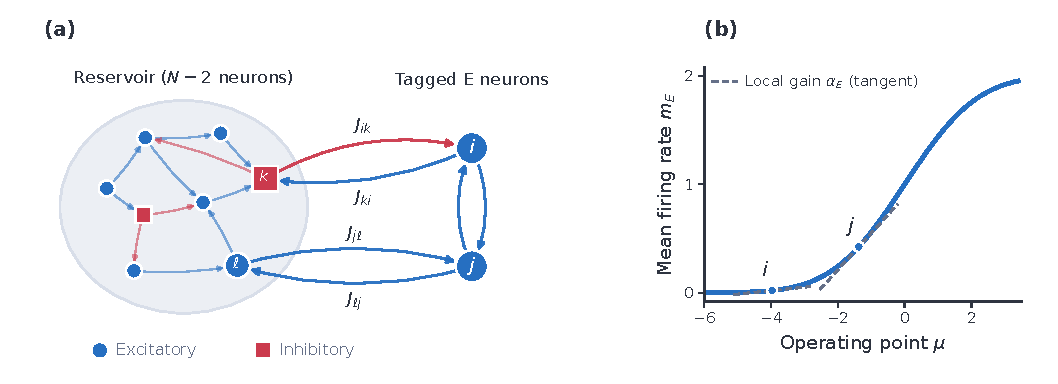
\includegraphics[width=\linewidth]{../docs/cavity_schematic.pdf}
\caption{\textbf{Two excitatory cells can have different local gains.}
The reservoir contains the other $N-2$ neurons. Each drawn edge takes its
sign from its presynaptic cell, so $J_{ik}$ carries the rate of cell $k$ to
cell $i$. Arrowheads end excitatory connections and flat bars end inhibitory
ones. The connections are schematic. The two points on the conditional
mean rate curve mark the lower and upper quartiles of the predicted E
operating-point distribution (gray density, arbitrary height) for the
Bernoulli reference in Eq.~\eqref{eq:reference}. At fixed $q_E$, their tangent slopes
are the local gains in Eq.~\eqref{eq:localerf}.}
\label{fig:cavity_sites}
\end{figure}

For independent edges, the one-site self-consistency equations are
\begin{align}
 \Delta_a&=\sum_bW_{ab}\E_z[m_b(z)^2],\label{eq:static}\\
 K_a''(\tau)&=K_a(\tau)-\sum_bW_{ab}\E_z c_b(z,\tau),\qquad
 K_a'(0)=0,\quad K_a(\infty)=0.
 \label{eq:dynamic}
\end{align}
Static input disorder survives at large $N$ because each row sums centered
couplings with total variance of order one. Its source includes
$\E m_b^2=\bar m_b^2+\operatorname{Var}_z m_b$; removing the latter term
would discard recurrently generated rate heterogeneity.

\begin{figure}[t]
\centering
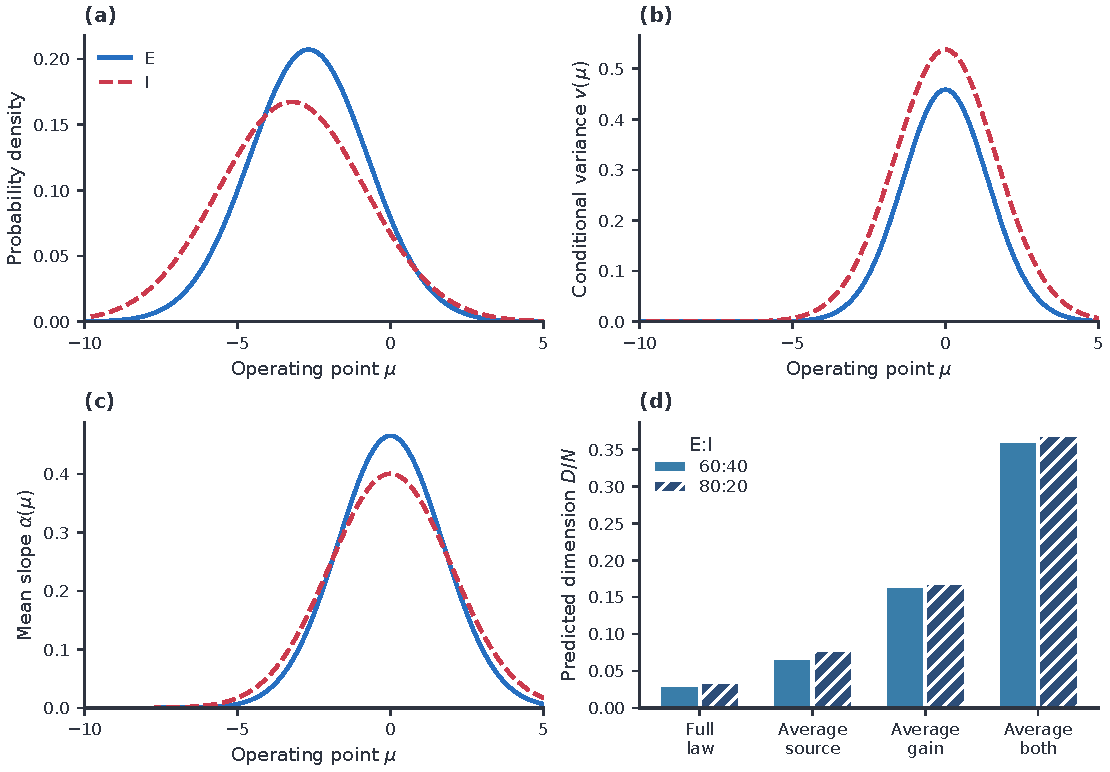
\includegraphics[width=\linewidth]{conditional_local_laws.pdf}
\caption{\textbf{The same operating point controls activity variance and response.}
(a) Predicted static operating-point distributions in the nonuniform EI
reference model. (b,c) Conditional temporal rate variance and local average
slope. The E and I laws differ, and neurons within either population sample
different parts of these curves. (d) Parameter-only dimension predictions
under two approximations to the same local law: average the conditional
spectra before forming their product, or replace $\E\alpha^2$ by
$(\E\alpha)^2$. Either approximation raises the predicted dimension.
The controls retain the original local covariances and PR numerator; they
are not new self-consistent network ensembles. The two compositions hold
$W=GF$ and $J^0F$ fixed. No network data or fitted amplitudes enter this figure.}
\label{fig:local}
\end{figure}

\section{A population response for covariance geometry}

Use the Fourier transform $c(\omega)=\int e^{-i\omega\tau}c(\tau)\dd\tau$,
with inverse measure $\dd\omega/(2\pi)$. The local response to additive
input current, before recurrent propagation, is
\begin{equation}
 s_a(z,\omega)=\alpha_a(z)H(\omega),\qquad
 H(\omega)=\frac{1}{1+i\omega}.
 \label{eq:response}
\end{equation}
At each pair of frequencies, retain the same neuronal label in the products
\begin{equation}
 Q_a(\omega_1,\omega_2)=\E_z[c_a(z,\omega_1)c_a(z,\omega_2)],\quad
 A_a=\E_z\alpha_a(z)^2,\quad
 U=H(\omega_1)H(\omega_2)\diag(A_a).
 \label{eq:source}
\end{equation}
The source $Q_a$ is not the product of two population-averaged spectra.
That distinction preserves the covariance of a neuron's two spectral factors.

In addition to the one-site law, the cavity closure assumes weak distinct-site
correlations, leading conditional decoupling of reservoir responses, and
bounded response and covariance norms at fixed parameters. Coherent EI
feedback must remain stable; an unstable or unusually amplified population
mode cannot be dropped on the grounds that the mean coupling has low rank.
Under these assumptions, define
\begin{equation}
 R=(I-UW)^{-1},\qquad \mathsf D_{\rm src}=\diag(Q_a/f_a),\qquad
 X=R\mathsf D_{\rm src}R^\dagger,\qquad \Psi=X-\mathsf D_{\rm src}.
 \label{eq:resolvent}
\end{equation}
Here $\Psi_{ab}$ is the scaled two-frequency product for distinct neurons
in populations $a,b$; $X$ restores the diagonal contributions. Algebraic
identities conditional on this closure are derived in Appendix~\ref{app:final_conditional_analytics}.

The integrated population contributions and dimension are
\begin{equation}
 \energy_{ab}=f_af_b\int\!\!\int X_{ab}(\omega_1,\omega_2)
                        \frac{\dd\omega_1\dd\omega_2}{(2\pi)^2},\qquad
 \energy=\sum_{ab}\energy_{ab},\qquad
 \boxed{\frac{\PR}{N}=\frac{(\sum_af_a\bar v_a)^2}{\energy}},
 \quad \bar v_a=\E_zv_a.
 \label{eq:geometry}
\end{equation}
The E--I contribution occurs twice in the total energy. It is a covariance
energy, not a participation ratio of a rectangular cross-covariance matrix.
For population $a$ alone,
\begin{equation}
 \frac{D_a}{N_a}=\frac{\bar v_a^2}
 {f_a\int\!\!\int X_{aa}\,\dd\omega_1\dd\omega_2/(2\pi)^2}.
 \label{eq:populationpr}
\end{equation}
Population PRs alone do not determine the alignment of E and I activity
subspaces.

An equivalent decomposition exposes two routes to low dimension:
\begin{equation}
 \energy=\sum_af_a\E_zv_a^2+\sum_{ab}f_af_b\psi_{ab},\qquad
 \psi_{ab}=\int\!\!\int\Psi_{ab}\frac{\dd\omega_1\dd\omega_2}{(2\pi)^2}.
 \label{eq:diagonal}
\end{equation}
Variance heterogeneity increases the diagonal second moment relative to the
squared mean variance, while pair correlations add off-diagonal energy.
Both must be retained before taking the PR ratio.
At fixed parameters with finite nonzero $\nu$ and $\energy$, the prediction
is extensive, $D\sim Nd$. Distinct pair covariances can vanish as
$N^{-1/2}$ while their $N^2$ squared contributions remain of order $N$,
the same order as the diagonal energy. Weak pair correlations therefore
change the leading dimensionality fraction rather than disappearing from
the collective observable.

\subsection{Relating E and I activity geometry}

A normalized cross-population energy isolates geometry from separate
population amplitude scales. For centered neuron-by-time activity matrices
$Y_a$, let $\mathsf K_a=Y_a^\top Y_a/T$ be their temporal Gram matrices.
Since $C_{ab}=Y_aY_b^\top/T$, cyclicity of trace gives
\begin{equation}
 \mathcal O_{EI}
 =\frac{\energy_{EI}}{\sqrt{\energy_{EE}\energy_{II}}}
 =\frac{\tr(\mathsf K_E\mathsf K_I)}
        {\|\mathsf K_E\|_F\|\mathsf K_I\|_F},\qquad
 0\leq\mathcal O_{EI}\leq1.
 \label{eq:temporalalignment}
\end{equation}
For nonzero Gram norms, this normalized Hilbert--Schmidt alignment is linear centered kernel
alignment for the time-centered activity matrices \citep{kornblith2019}.
It is invariant under a separate common rescaling of all E rates or all I
rates. It compares population temporal Gram geometry, rather than defining
a communication dimension or a PR of the rectangular cross block.
The simulations estimate its stationary energies through the corrected
window products described below. The finite-record ratio is not exactly
unbiased and need not obey the population bound on every estimate.

Let $t_a=\tr C_{aa}$ and $w_a=t_a/(t_E+t_I)$ be fractions of temporal
variance. With absolute population dimensions $D_E,D_I$, the exact identity
\begin{equation}
 \boxed{\frac1D=\frac{w_E^2}{D_E}+\frac{w_I^2}{D_I}
      +\frac{2\mathcal O_{EI}w_Ew_I}{\sqrt{D_ED_I}}}
 \label{eq:jointgeometry}
\end{equation}
relates population and joint dimensionality. The weights $w_a$ are variance
fractions, not neuron fractions $f_a$. Equal population dimensions $D_0$
give joint dimension $D_0$ at perfect Gram overlap; at zero overlap and equal
variance fractions, they give $2D_0$. The conditional pair theory predicts
all the terms of this geometric relation.

\subsection{Why averaging too early raises dimension}

For common leak times, set $B=\diag(A)W$ and assume $B$ is nonnegative with
$\rho(B)<1$. Expanding both resolvents gives
\begin{equation}
 \int\!\!\int X_{ab}\frac{\dd\omega_1\dd\omega_2}{(2\pi)^2}
 =\sum_{c,n,m\geq0}\frac{(B^n)_{ac}(B^m)_{bc}}{f_c}
   \E_z[a_{nm,c}(z)^2],
 \label{eq:averagingseries}
\end{equation}
where
$a_{nm,c}(z)=\int c_c(z,\omega)H(\omega)^nH(\omega)^{*m}
\dd\omega/(2\pi)$ is real by conjugate symmetry. The interchange requires
integrable spectra and a dominated convergent series.

\begin{proposition}[Conditional averaging]
Under these assumptions and with the local-law numerator held fixed,
replacing $Q_c$ by the product of averaged spectra cannot increase any
integrated population covariance energy. Replacing $A_a=\E\alpha_a^2$ by
$(\E\alpha_a)^2$ also cannot increase these energies. Either replacement
therefore cannot decrease the predicted total or within-population PR.
\end{proposition}
For the first statement, Eq.~\eqref{eq:averagingseries} replaces a second
moment by a squared mean, with nonnegative coefficients. For the second,
Jensen's inequality lowers $B$ entrywise and hence lowers every coefficient
in the series. Figure~\ref{fig:local} shows that these effects are substantial
for the reference EI law. The proposition compares approximations to a fixed
conditional law; it does not impose an ordering on arbitrary biological
interventions that also change that law.
The mechanism has two parts. Neurons with large local slopes contribute
disproportionately to repeated recurrent propagation, so averaging the slopes
before taking response moments removes that amplification. At the same time,
each neuron's covariance contributes a product of its own spectral factors;
averaging the spectra first removes a nonnegative source of covariance
energy. Neither effect is determined by the mean firing rate alone.

\section{Two distinct connectivity interventions}

\subsection{Population composition at fixed aggregate input}

Rescale presynaptic columns so that $J^0F$ and $W=GF$ remain fixed while $f$
changes. Equations~\eqref{eq:balance}--\eqref{eq:dynamic} then preserve the
one-site laws within the theory. The source weights $1/f_a$ and population
weights $f_af_b$ still change. In particular, with the fraction-independent
tensor
\begin{equation}
 T_{abc}=\int\!\!\int R_{ac}R_{bc}^*Q_c
                    \frac{\dd\omega_1\dd\omega_2}{(2\pi)^2},
 \qquad
 \energy_{ab}=f_af_b\sum_c\frac{T_{abc}}{f_c},
 \label{eq:composition}
\end{equation}
one conditional calculation predicts the entire controlled fraction family.
For the reference local law, changing the fraction from 80:20 to 60:40
raises the predicted share $2\energy_{EI}/\energy$ from $0.305$ to $0.448$,
despite preserving the conditional local laws. Population geometry is
therefore a distinct prediction even when the change in total PR is modest.
Holding individual edge moments fixed defines a different intervention and
requires recomputing the local laws. No biological optimum follows from
an optimum along one such parameter path.
The numerical reference has
\begin{equation}
 G^0=\begin{pmatrix}16&9\\25&12\end{pmatrix},\qquad
 J^{0,\rm ref}=\begin{pmatrix}1&-6\\2&-10\end{pmatrix},\qquad
 f^0=(0.8,0.2),\qquad \bar m=(0.3,0.3).
 \label{eq:reference}
\end{equation}
The required leading drive is $I=(0.12,0.12)$. Changing composition rescales
each presynaptic column of both matrices by $f_b^0/f_b$. The resulting
Bernoulli probabilities are $p_{ab}=(J^0_{ab})^2/[G_{ab}+(J^0_{ab})^2]$,
with $t_{ab}=J^0_{ab}/p_{ab}$. The ensemble includes self-connections.

\subsection{Degree dispersion at fixed edge marginals}

For each incoming population block of size $M=N_b$, draw a count $K_{ab}$
with mean $Mp_{ab}$ and choose that many presynaptic neurons uniformly.
Different incoming rows and presynaptic classes are independent. Define
\begin{equation}
 \chi_{ab}=\frac{\operatorname{Var}K_{ab}}{Mp_{ab}(1-p_{ab})}.
 \label{eq:chi}
\end{equation}
Bernoulli edges have $\chi=1$; fixed integer counts have $\chi=0$.
This control preserves each edge's marginal mean and variance, but changes
correlations between edges in a row. The exact finite-pool sampling identity
then gives the leading static equation
\begin{equation}
 \boxed{\Delta_a=\sum_bW_{ab}
 [\operatorname{Var}_z m_b(z)+\chi_{ab}\bar m_b^2].}
 \label{eq:degreestatic}
\end{equation}
Fixed counts remove the disorder caused by sampling different numbers of
neurons with a common mean rate. They leave disorder from sampling unequal
presynaptic mean rates. The same distinction was identified in EI mean-field
comparisons of fixed and stochastic in-degree \citep{mastrogiuseppe2017}.
For fixed nonzero dispersion, count deviations are of order $\sqrt M$.
Multiplying by a synapse of order $N^{-1/2}$ and a nonzero mean rate leaves
an order-one quenched input offset even as relative count fluctuations
vanish. This persistent static disorder is consistent with concentration
of the centered temporal input kernel in the limiting closure.
Within-row coupling covariances are only of order $N^{-2}$, but their
contribution to static input sums over order $N^2$ pairs of presynaptic mean
rates. Degree constraints can therefore change static disorder by order one
while preserving every edge marginal. This change then propagates through
the conditional nonlinear responses into collective geometry.

For bounded dispersion and growing in-degree, the dynamic and pair equations
retain their leading form under the stated asynchronous and stable-coherent
assumptions, after the conditional law is recomputed. Our nonuniform degree
test measures this prediction where the E and I local laws differ. It also
records the generator's actual dispersion, since integer rounding is part
of a finite-network intervention.
In this controlled family, the leading drive $\sqrt N I$ and the edge-moment
matrices remain fixed, while the order-one drive is set to the residual
input $h_a(\chi)$ computed from the parameter-only conditional theory. Thus
the stated intervention does not keep the entire external drive fixed; the
order-one change is prescribed before measuring the networks and is not a
fit to their PR.
To separate variance heterogeneity from pair correlations, set
$\energy_{\rm diag}=\sum_af_a\E v_a^2$. Then
\begin{equation}
 d=\underbrace{\frac{\nu^2}{\energy_{\rm diag}}}
                 _{\text{variance heterogeneity}}
   \underbrace{\frac{\energy_{\rm diag}}{\energy}}
                 _{\text{pair correlations}}.
 \label{eq:degreefactors}
\end{equation}
For the ideal nonuniform degree control from $\chi=0$ to $\chi=2$, these
parameter-only factors fall by 2.93-fold and 3.53-fold, respectively, giving
a 10.34-fold predicted reduction in $d$. Thus the predicted degree effect
changes activity geometry as well as its overall amplitude; common covariance
rescaling would leave PR invariant.

\section{Network tests and the validity of the closure}
\label{sec:results}

\subsection{Separate recording bias from the dynamical prediction}

The fraction diagnostic was motivated by two 60:40, $N=1000$ realizations
whose original dimension estimates were approximately $0.0135$ and $0.0141$,
against the leading prediction $0.0299$. A pair of unusual networks does
not establish an ensemble bias, and finite-record corrections must be
distinguished from connectivity variation.

The limiting theory predicts infinite-time, neuron-wise centered covariance.
Subtracting a separate empirical mean in each recording block changes that
observable. Appendix~\ref{app:recording} gives an exact mean-difference repair
for independent stationary windows; duration and gap checks test the residual
dependence between windows in actual trajectories.

The existing sixteen-network 60:40 Bernoulli cohort was extended from 4000
to 16000 recorded leak times, preserving each connectivity realization and
initial condition. The original primary-prefix statistics reproduce to
floating-point precision. The standard eight-block estimate changes from
$d=0.027281$ to $0.026041$. At the longer duration, the mean-difference
estimate is $0.025678$ with network standard error $0.001627$ for block
length 500 and a one-block empty gap. Block lengths 1000 and 2000 give
$0.025681$ and $0.025600$ under the corresponding historical gap choice.
The standard-minus-corrected differences decrease approximately as the
inverse block length. This agreement among corrected block choices supports
the estimator repair; it does not prove infinite-time convergence.

The leading parameter-only prediction is $0.029894$, while the retained
formal first-order correction gives $0.030871$ at $N=1000$. Thus the
expanded historical cohort weakens the original factor-two mismatch but
does not establish quantitative agreement. The selected historical seeds
and remaining time and state effects restrict the interpretation of a
network-mean interval. The new prospective comparisons below use fresh
connectivity realizations under a shared estimator protocol.
In this historical cohort, the mean numerator moment is 5.8\% below its
leading value and the mean covariance energy is 9.3\% above. Their
ratio-of-means dimension is approximately $0.02427$, below the mean of
network ratios $0.02568$, as required by Eq.~\eqref{eq:ratiobias}.
This accounting locates the residual in the ingredients; it is not a
parameter-only explanation of why those finite-network shifts occur.

\begin{figure}[t]
\centering
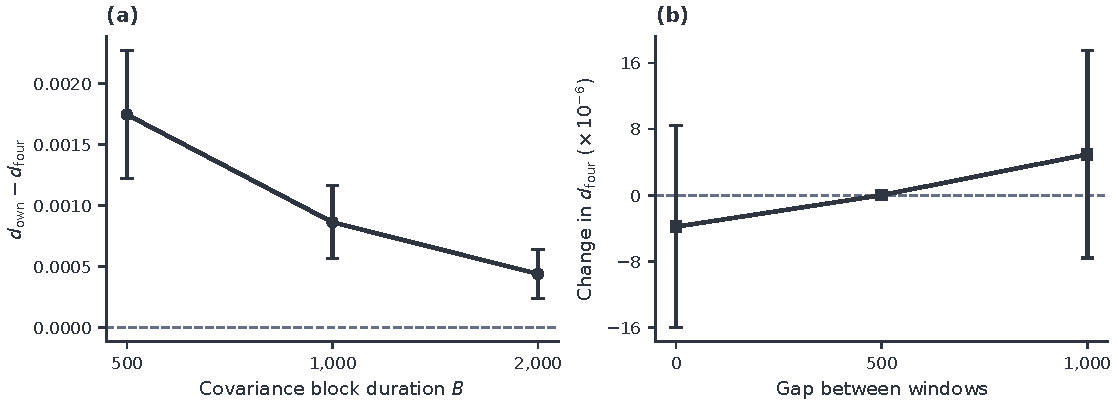
\includegraphics[width=\linewidth]{finite_record_diagnostics.pdf}
\caption{\textbf{Separated windows do not remove their own centering bias.}
Historical sixteen-network Bernoulli 60:40 cohort, $N=1000$, extended to
16000 recorded leak times. (a) The standard separately centered estimate
exceeds the mean-difference estimate at the same block length. Increasing
duration while holding block length fixed does not remove this contribution.
(b) After the repair, changing the minimum empty gap from zero to 1000 leak
times at block length 500 changes mean PR by only a few parts in $10^6$ in
this cohort. Error bars are 95\% Student-$t$ intervals of paired differences
across connectivity realizations; overlapping window quadruples are not
independent network replicates. The panels have different vertical scales.
These checks support this parameter point, not a uniform mixing theorem.}
\label{fig:recording}
\end{figure}

\subsection{The nonuniform degree intervention produces a large dimensionality change}

The degree test uses the nonuniform reference matrices in
Eq.~\eqref{eq:reference}, so that E and I have different local kernels.
The initial eighteen-network allocation contains three fresh connectivity
draws at each of four dispersions for $N=1000$, and three at each endpoint
for $N=2000$. After the quantitative deviations at the larger size, a staged
extension allocated three $N=4000$ networks at each endpoint before observing
those outcomes. All twenty-four networks from this original cohort are retained
in Table~\ref{tab:degree}. Endpoint mean dimensions differ by factors
$7.87$, $7.13$, and $8.41$ at the three sizes, compared with the
parameter-only prediction $10.34$. Thus the large degree effect transfers
to a genuinely nonuniform population profile.

\begin{table}[t]
\centering
\caption{Nonuniform degree test. Measurements are network means with
standard errors. The theoretical value is the ideal requested-dispersion
prediction; integer-count rounding is recorded separately. The initial 18
networks and the staged six-network extension are distinguished in the text.}
\label{tab:degree}
\begin{tabular}{rrrrrr}
\toprule
$N$&$\chi$&$n$&Predicted $d$&Measured $d$&Network SE\\
\midrule
1000&0&3&0.173891&0.149156&0.003542\\
1000&0.5&3&0.055942&0.041364&0.004108\\
1000&1&3&0.034326&0.030165&0.002399\\
1000&2&3&0.016811&0.018960&0.000788\\
2000&0&3&0.173891&0.156176&0.001276\\
2000&2&3&0.016811&0.021896&0.000997\\
4000&0&3&0.173891&0.162277&0.001482\\
4000&2&3&0.016811&0.019306&0.001620\\
\bottomrule
\end{tabular}
\end{table}


In the original cohort, the quantitative discrepancies also transfer. The $N=2000$ endpoint means
are $10.2\%$ below and $30.3\%$ above their respective predictions.
At $N=4000$, these discrepancies are $-6.7\%$ and $+14.8\%$; the
temporal-input-variance errors are about $3.3$--$4.3\%$ across the two
populations and endpoint conditions.
Figure~\ref{fig:degree} displays the local input statistics and absolute
population covariance energies alongside PR. These ingredients show
departures from the limiting law, so the residual cannot be assigned to a
PR ratio alone. Increasing size does not uniformly improve every comparison.
Sensitivity of mean PR to the tested duration and gap choices is only a few
$10^{-4}$ at these degree points: the largest gap shift is $0.000131$ and
the largest 4000-to-8000 duration shift is $0.000461$. Re-solving the conditional equations at
the generator's expected rounded dispersion, while reimposing target means,
changes predicted PR by less than $0.74\%$; this retargeted diagnostic is
kept separate from the primary prediction and is too small to repair the
observed discrepancies.

The follow-up tested twelve dispersions at $N=2000$ with three new networks
at each setting. Three $N=4000$ networks at each of $\chi=0.1,0.75,1.5$
checked selected interior points. In the new $N=2000$ cohort, mean $D/N$
fell from $0.1540$ to $0.0187$ across the endpoints (an 8.24-fold change).
Among the sampled dispersions the largest mean E--E and twice-E--I block
energies occurred at $\chi=0.5$ and $\chi=0.3$, respectively. After four
measurements from the first seed became available, we defined a supplemental
test at the eight dispersions absent from the original sweep. We compared the
root-mean-square error in $\log(D/N)$ for the conditional curve and for the
straight line joining its theoretical endpoints in these coordinates. For
the two independent seeds measured after we chose the test, the errors were
$0.141$ versus $0.455$ and $0.131$ versus $0.428$, respectively. Across all
three seeds, the mean errors were $0.134$ and $0.443$. The descriptive paired
difference was $-0.310$ (95\% interval $[-0.337,-0.282]$).

\begin{figure}[t]
\centering
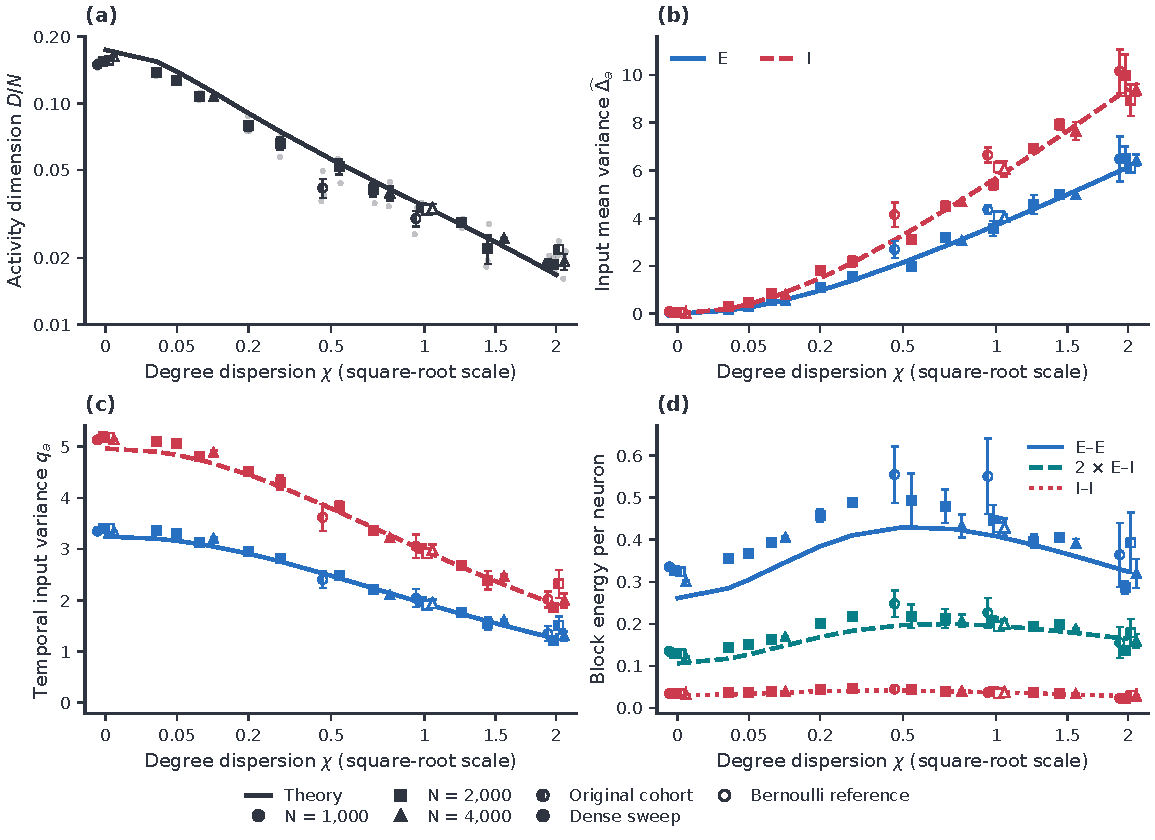
\includegraphics[width=\linewidth]{degree_validation.pdf}
\caption{\textbf{Degree dispersion changes local input statistics and covariance geometry.}
At 80:20 E:I, (a) shows joint dimension per neuron, (b) the across-neuron variance
of finite-record input means, (c) the temporal input variance, and (d) the E--E,
twice E--I, and I--I covariance energies per network neuron. Lines give the
conditional predictions. The square-root scale resolves the closely spaced
dispersions near zero. Marker shape identifies network size. Half-filled symbols
summarize the original 24 networks and filled symbols the 45 new networks.
Each cohort, size, and dispersion has its own mean and one across-network
standard error. Faint dots in (a) are individual realizations. Hollow symbols
at $\chi=1$ give separate Bernoulli references from 12 networks at $N=2000$
and four at $N=4000$. All estimates use 8000 recorded leak times.
The raw input means in (b) retain finite-time sampling noise.}
\label{fig:degree}
\end{figure}

\subsection{Composition and size separate population allocation from absolute accuracy}

The original size series was staged. The initial allocation includes four seed
clusters per composition at $N=1000$ and $N=2000$; after the pilot spread,
the allocation adds eight per composition at $N=2000$ and four per
composition at $N=4000$. Each stage is recorded before its outcomes, every
realization is retained, and first-stage versus additional-seed results are
kept separately. The main observables are $\nu$, $\energy$, $d$, and absolute
population energies. The normalized geometry diagnostics below are
exploratory secondary observables.

In the original $N=2000$ size series, each composition contributed twelve realizations.
The 60:40 means are $\nu=0.151999$, $\energy=0.795195$, and $d=0.029417$,
with relative discrepancies $-0.60\%$, $+1.65\%$, and $-1.59\%$.
The corresponding 80:20 discrepancies are $-1.15\%$, $+2.85\%$, and
$-3.40\%$. For the 60:40 mean dimension, the conventional 95\% relative-error
interval is $[-9.80\%,+6.61\%]$; for 80:20 it is
$[-12.58\%,+5.78\%]$. Across all six moment and dimension means at this
size, interval endpoints range from $-12.58\%$ to $+14.19\%$.
These are descriptive finite-record sampling intervals at the tested
coupling and compositions. They do not bound individual realizations,
establish uniform convergence, or extend the same accuracy to all degree
conditions.
At $N=4000$, the four-network means are $d=0.029973$ at 60:40 and
$d=0.033491$ at 80:20, with relative discrepancies $+0.27\%$ and
$-2.43\%$. Their mean-error intervals are
$[-4.72\%,+5.25\%]$ and $[-17.55\%,+12.68\%]$.
The 60:40 mean numerator and energy are $5.11\%$ and $10.52\%$ above
their leading values; the energy-error interval spans
$[-9.28\%,+30.32\%]$. Thus stable PR does not establish monotone
convergence of the amplitudes or a controlled cancellation of all missing
terms. The more precise $N=2000$ ingredient comparison remains independent
evidence alongside the largest-size PR check.

\begin{table}[t]
\centering
\caption{Fresh composition and size series. Ratios compare the mean of each
network observable with its parameter-only prediction. The interval is a
conventional 95\% Student-$t$ interval for the mean dimension ratio across
independent seed clusters within each condition; it does not include
uncontrolled finite-record bias or provide simultaneous coverage. The
staged allocation and every outcome are retained.}
\label{tab:composition}
\begin{tabular}{rrrrrrr}
\toprule
$f_E$&$N$&$n$&$\bar\nu/\nu_0$&$\bar\energy/\energy_0$&$\bar d/d_0$&95\% interval\\
\midrule
0.6&1000&4&0.869&0.945&0.806&$[0.470,1.142]$\\
0.8&1000&4&0.975&1.100&0.883&$[0.250,1.517]$\\
0.6&2000&12&0.994&1.017&0.984&$[0.902,1.066]$\\
0.8&2000&12&0.988&1.029&0.966&$[0.874,1.058]$\\
0.6&4000&4&1.051&1.105&1.003&$[0.953,1.053]$\\
0.8&4000&4&1.007&1.041&0.976&$[0.825,1.127]$\\
\bottomrule
\end{tabular}
\end{table}


The temporal Gram alignment provides a complementary geometry test.
At $N=2000$, its mean is $0.87217$ at 60:40 and $0.78920$ at 80:20,
against parameter-only values $0.87364$ and $0.79054$. These mean
relative discrepancies are about $0.17\%$, with no fitted population amplitude.
Normalized allocation of total energy to E--E, E--I, and I--I differs from
the predicted matrix by $1.37\%$ and $2.31\%$ in relative Frobenius norm.
This last statistic compares the ensemble mean of normalized matrices;
the ratio of ensemble mean energies is retained separately. Agreement of
these normalized observables does not eliminate errors in absolute energy.
At $N=4000$, mean alignments are $0.87224$ and $0.78907$, while the
normalized allocation-matrix discrepancies are $0.64\%$ and $0.91\%$.
The relative geometry remains close even when an overall energy error grows.

\begin{figure}[t]
\centering
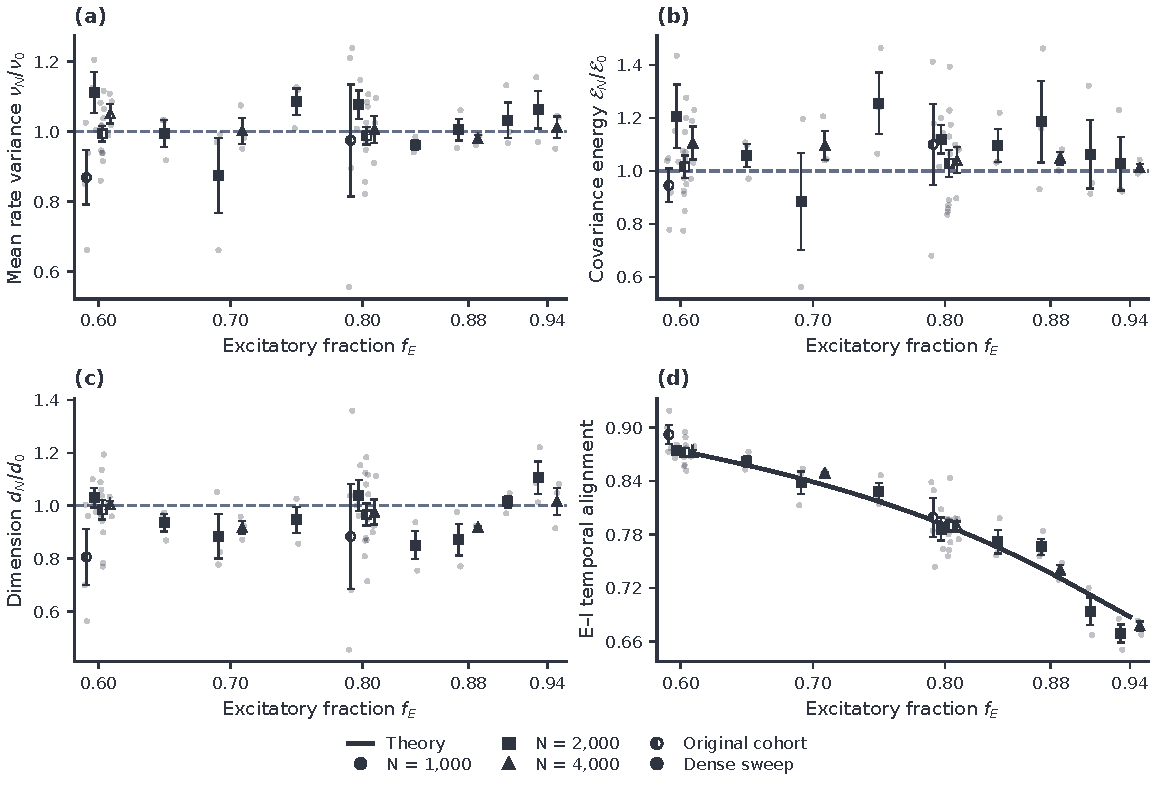
\includegraphics[width=\linewidth]{composition_main.pdf}
\caption{\textbf{Composition changes temporal alignment and the accuracy of the predicted moments.}
The excitatory fraction varies at fixed $J^{0}F$, $GF$, target rates and $\chi=1$.
(a--c) The mean rate variance, covariance energy and joint dimension are divided
by their conditional predictions at each fraction. Dashed lines mark one.
(d) The solid line predicts temporal Gram alignment,
$\mathcal O_{EI}=\energy_{EI}/\sqrt{\energy_{EE}\energy_{II}}$.
Half-filled symbols summarize the original 40 networks at 60:40 and 80:20 E:I.
Filled symbols summarize 36 new networks spanning nine fractions at $N=2000$
and three at $N=4000$, with three connectivity draws at each size and fraction.
Points and bars show individual draws and means with one across-network
standard error. Symbols at the same fraction are offset horizontally.}
\label{fig:composition}
\end{figure}

The composition follow-up sampled $f_E=0.60,0.65,0.70,0.75,0.80,0.84,0.88,
0.91,0.94$ at $N=2000$ and $f_E=0.70,0.88,0.94$ at $N=4000$.
Each setting had three new connectivity seed labels, reused across fractions
for paired comparisons. To compare within-population covariance per available
pair across fractions, we exclude self-pairs and normalize by the number of
distinct ordered pairs.
\begin{equation*}
 P_{aa}=\frac{N}{N_a(N_a-1)}\sum_{\substack{i,j\in a\\i\ne j}} C_{ij}(0)^2,
 \qquad \frac{D_E}{N}=f_E\frac{D_E}{N_E}.
\end{equation*}
The second quantity counts E dimensions at a fixed total network size. For the
fixed aggregate couplings, the theory predicts a maximum of $D_E/N$ at $f_E=0.887$ and minima of the distinct-pair
energies $P_{EE}$ at $0.882$ and $P_{II}$ at $0.768$
(Fig.~\ref{fig:population_sweep}). From $f_E=0.80$ to $0.88$ at $N=2000$,
the paired mean changes in $P_{EE}$ and $P_{II}$ were $+0.002$ (95\% interval
$[-0.325,+0.329]$) and $+0.236$ (95\% interval $[-0.386,+0.858]$).
Both intervals include zero, so these measurements leave the proposed E--E
decrease and I--I increase unresolved.
For $D_E/N$, the pointwise 95\% intervals on the paired changes were
$[-1.97,+1.23]$ percentage points between 0.80 and 0.88 and $[-0.96,+2.16]$ percentage points between 0.88 and 0.94.
The corresponding 0.88-to-0.94 interval at $N=4000$ was $[-0.57,+0.93]$ percentage points.
Each interval uses three matched seed differences. The sampled changes leave the location of an empirical maximum unresolved.

\begin{figure}[t]
\centering
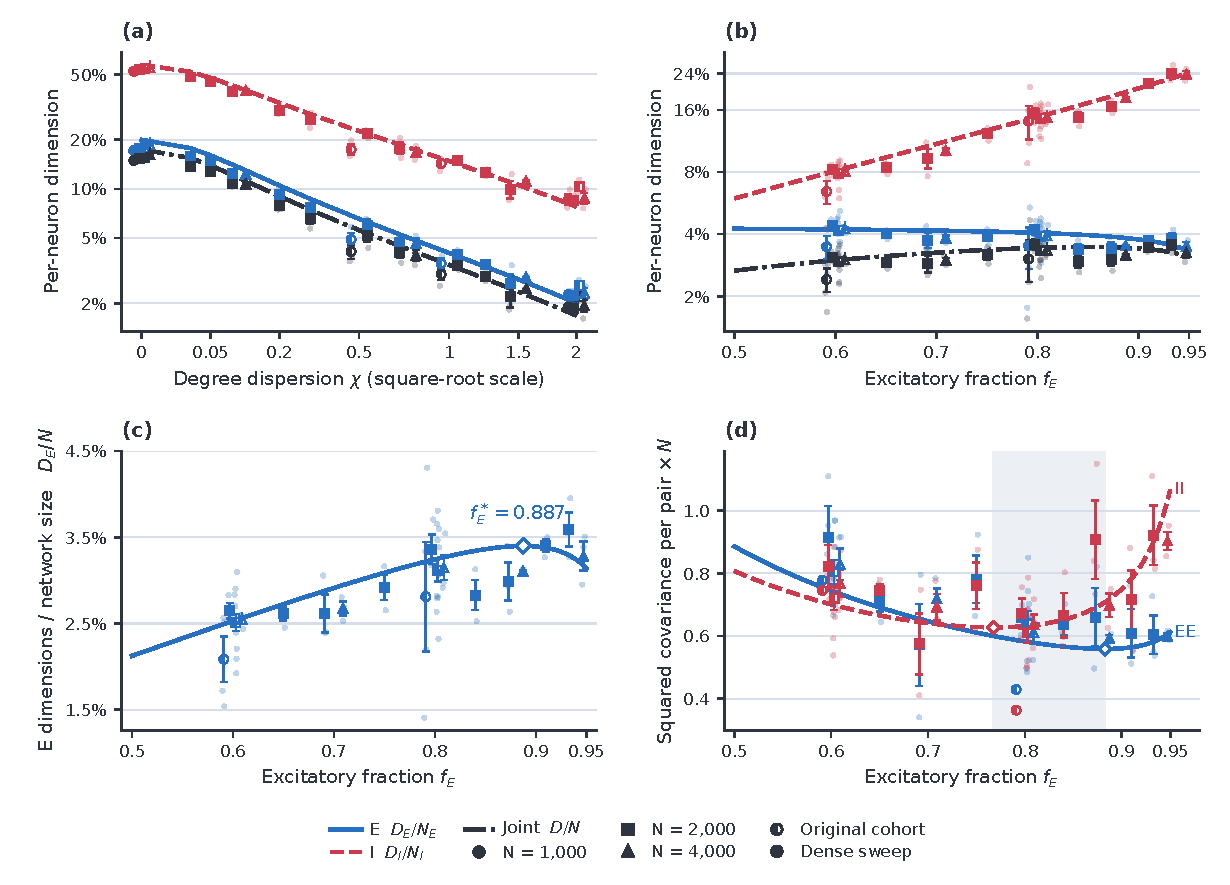
\includegraphics[width=\linewidth]{../figures/population_pr.pdf}
\caption{\textbf{Composition separates per-neuron dimension from total E dimension.}
(a) E-only, I-only and joint participation ratios per corresponding
neuron as degree dispersion changes at 80:20 E:I (square-root horizontal scale).
(b) The same dimensions against excitatory fraction at fixed aggregate couplings
and $\chi=1$. (c) E dimension per network neuron, $D_E/N$. (d) $P_{aa}$,
the mean squared covariance over distinct ordered pairs in population $a$ multiplied
by $N$. Hollow diamonds mark the theoretical extrema. In the shaded interval,
the theory predicts falling $P_{EE}$ and rising $P_{II}$. Faint dots show
networks. Means and one standard error are computed within a cohort, size and
setting. The 69 degree networks enter (a), and all 76 composition networks
enter (b,c). Matched diagonal and block energies are available for 64 of the
composition networks in (d).}
\label{fig:population_sweep}
\end{figure}

The two averaging controls distinguish what these observables test. At
80:20, averaging the gains predicts $\mathcal O_{EI}=0.35138$ instead of
$0.79054$. Averaging the source spectra retains nearly the same alignment,
$0.78766$, but predicts $d=0.07645$ instead of $0.03433$. At $N=2000$, the
measured mean in the original cohort is $0.03316$. Thus alignment alone is insensitive to an
important source-moment approximation, while joint dimensionality and
alignment constrain both response and source heterogeneity. These remain
approximations to the fixed local law, not retuned homogeneous networks.

Population PR illustrates the need to distinguish neuron counts from
absolute dimension. In the original cohort at 80:20 and $N=2000$, the measured per-neuron fractions
are $D_E/N_E=0.03898$ and $D_I/N_I=0.14525$, while their absolute dimensions
are $62.38$ and $58.10$. At 60:40 the absolute values are $50.24$ and
$63.12$. Population dimensions therefore do not simply add to obtain the
whole-network dimension; Eq.~\eqref{eq:jointgeometry} supplies the missing
variance weights and temporal overlap.
Table~\ref{tab:population_dimensions} reports per-neuron and absolute
population dimensions separately.

An ingredient residual remains: the mean squared time-averaged gains at
$N=2000$ lie about $6$--$8\%$ below their predictions. Diagnostic
substitution of measured individual means and temporal variances predicts
the measured gain moment to within about $1\%$ on nine instrumented
networks per composition, while a population Gaussian approximation using
measured $(h,\Delta,q)$ overestimates it by roughly $5$--$8\%$.
Cross-block gain-product checks change the estimate by less than $0.1\%$.
The intermediate substitution of empirical operating points with a common
temporal variance leaves errors of roughly $1.6$--$4.4\%$. Thus both
substitutions reduce the residual in this prescribed diagnostic order.
This locates the dominant tested gain residual in the operating-point
distribution and common-variance approximation, rather than the numerical
gain estimator. It tests the conditional Gaussian one-time marginal mapping,
not the full Gaussian trajectory law. Such same-record calibrated checks are
kept separate from the parameter-only prediction. The good agreement in trace moments and relative
geometry does not establish uniform accuracy of all one-site statistics or
control of the formal finite-size expansion.
At $N=4000$, measured gain moments remain roughly $4$--$7\%$ below
prediction, whereas the empirical individual-moment
calibration errors remain below $0.6\%$ in magnitude. The corresponding
population-Gaussian calibration errors are $3.1$--$5.7\%$
(Table~\ref{tab:gain_calibration}).

Selected step refinements and tangent checks are given in
Appendix~\ref{app:integration_checks}. Four selected PR changes are below
$1.1\%$, but one 80:20, $N=1000$ realization changes by $24.3\%$ and
remains a material sensitivity. A same-step backend change shifts its
8000-time PR by $17.7\%$, and three refined native 16000-time runs still
span $12.3\%$. The tests do not uniquely attribute the discrepancy to
step truncation or establish a converged invariant covariance for this
outlier. The primary outcome is retained. Numerical error therefore cannot be declared uniformly
negligible from these selected checks or from agreement of a PR ratio alone.

The original factor-two 60:40 mismatch does not persist in the tested
larger-network ensemble mean PR. The $N=1000$ deficit remains a
finite-network prediction limitation, with unresolved individual-network
recording and numerical sensitivity; the formal first correction does not
repair it. The
supported resolution is an empirical regime for the ensemble geometry
prediction with a checked recording protocol, rather than a universal
finite-$N$ correction or exact prediction of each circuit.

\subsection{Static and temporal variance must be tested separately}

A finite network can place more input variance in fixed differences between
neurons and less in temporal fluctuations. Testing only the total input
variance $V_a=\Delta_a+q_a$ would miss this change. Let
$\mathcal M_2(h,V,k)=\E[\phi(X_1)\phi(X_2)]$ for two Gaussian variables
with common mean $h$, marginal variance $V$, and covariance $k$. The
conditional Gaussian construction gives
\begin{equation}
 \bar v_a=\mathcal M_2(h_a,V_a,V_a)
          -\mathcal M_2(h_a,V_a,\Delta_a),\qquad
 \left.\frac{\partial\bar v_a}{\partial\Delta_a}\right|_{V_a,h_a}
 =-A_a.
 \label{eq:partitionderivative}
\end{equation}
The second identity follows from Gaussian integration by parts: differentiating
the shared covariance gives $\E[\phi'(X_1)\phi'(X_2)]$, which equals
$\E_z\alpha_a(z)^2=A_a$ at shared covariance $\Delta_a$.
Thus reallocating input variance toward static disorder lowers the temporal
rate variance along this specified diagnostic direction.

At fixed $V,h$, linearizing the static self-consistency functional gives the
susceptibility $(I-W\diag(A))^{-1}$. Its Perron-mode amplification is about
$6.94$ for the reference law. This sensitivity explains why modest changes
in local operating points can matter appreciably for activity fluctuations.
Actual networks also change $V$ and $h$, and the covariance energy changes
through both its source and its response. These derivative identities
therefore diagnose a possible finite-network mechanism; they do not supply
a complete correction to PR.



\section{Discussion}

The useful reduction is a map from a self-consistent distribution of local
trajectory laws to a small population response problem. Balance supplies
the distribution; the two-site calculation supplies covariance energy.
Their conditional combination preserves information that is lost in a
population-average neuron. Composition and degree variability act on
different parts of this map, providing separate tests of its structure.

Three qualifications limit its interpretation. First, the closure assumes
conditional cavity decoupling and controlled coherent feedback; the matrix
identity does not prove these properties for the nonlinear network. Second,
PR can conceal errors through correlated numerator and denominator shifts.
For any positive covariance-energy random variable,
\begin{equation}
 \E\frac{\nu^2}{\energy}-\frac{(\E\nu)^2}{\E\energy}
 =\E\frac{(\nu-a\energy)^2}{\energy}\geq0,\qquad
 a=\frac{\E\nu}{\E\energy}.
 \label{eq:ratiobias}
\end{equation}
We therefore report both ensemble summaries and their ingredients. Third,
finite recordings estimate a different object unless their centering and
mixing errors are controlled. The recording checks are part of validating
the observable, rather than a fit to the dynamical prediction.

The formal $N^{-1/2}$ stationary correction retained in the research archive
does not provide a controlled expansion at $N=1000$. Its known higher-order
resummations omit irreducible terms, and a small final PR shift does not
establish that large ingredient corrections are controlled. Completing the
full finite-size expansion is distinct from defining and testing the leading
conditional theory. Likewise, selected examples of weak chaos, fixed points,
and periodic activity establish a classification issue, not their ensemble
probabilities.
A concentration diagnostic can also depend on the effective dimension of
the presynaptic covariance after leak filtering and variance weighting,
rather than on $N$ alone. Appendix~\ref{sec:source-concentration-diagnostic}
gives the exact frozen-Gaussian-row identity. Its effective source dimension
is distinct from activity PR, and omitted degree constraints, cumulants,
endogenous conditioning, and coherent reinsertion prevent treating it as a
complete finite-network error bound.

Near a simple smooth instability, the conditional equations also admit a
critical-mode reduction. Nonzero local curvature generically produces a
three-halves dimension law; curvature can arise from a biased homogeneous
operating point as well as from quenched heterogeneity. The scalar
disorder--curvature crossover derived in the archive is therefore a
supporting analytical result, with finite-network visibility and the
nonuniform EI extension requiring their own evidence. It is not used to
replace the finite-coupling tests reported here.

\clearpage
\appendix
% Self-contained appendix input. Requires amsmath, amssymb only.
% No document class, bibliography commands, or project-specific macros.
\section{Conditional EI analytics and the population geometry}
\label{app:final_conditional_analytics}

This appendix completes the algebra of the conditional construction used in
this paper. The construction is an asymptotic cavity closure. Exact
finite-dimensional identities, algebraic implications of that closure, and
additional assumptions about the nonlinear network are kept separate. The
finite-network tests determine where the resulting parameter-only prediction
is quantitatively useful.

\subsection{Model, averaging operations, and the observable}

Let $i\in a$ identify a neuron in population $a$, with $N_a=f_aN$ and
$\sum_a f_a=1$. Set $F=\operatorname{diag}(f_a)$. In common leak-time units,
\begin{equation}
 \dot x_i=-x_i+\sum_jJ_{ij}\phi(x_j)+\sqrt N I_a+h_a^{\rm ext},
 \qquad \phi(x)=2\Phi(x),\qquad r_i=\phi(x_i).
 \label{eq:an_model}
\end{equation}
The dense Bernoulli ensemble has $J_{ij}=t_{ab}A_{ij}/\sqrt N$,
$t_{aE}>0$, $t_{aI}<0$, and independent $A_{ij}$ with success probability
$p_{ab}$. Its moment coefficients are
$J^0_{ab}=p_{ab}t_{ab}$ and $G_{ab}=p_{ab}(1-p_{ab})t_{ab}^2$.
Thus $\mathbb E J_{ij}=J^0_{ab}/\sqrt N$ and
$\operatorname{Var}J_{ij}=G_{ab}/N$. Self-connections follow the same rule.
Degree-constrained rows are treated below.

Time averaging within a stationary state is denoted by angle brackets;
$\mathbb E_z$ averages fixed neuronal operating points, and an ensemble average
over connectivity realizations is a further operation. Define
\begin{align}
 m_i&=\langle r_i\rangle,&
 C_{ij}(\tau)&=\langle[r_i(t+\tau)-m_i][r_j(t)-m_j]\rangle,\\
 \nu_N&=\frac{\operatorname{tr}C(0)}N,&
 \mathcal E_N&=\frac{\operatorname{tr}[C(0)^2]}N,&
 d_N&=\frac{D_{{\rm PR},N}}N=\frac{\nu_N^2}{\mathcal E_N}.
 \label{eq:an_observables}
\end{align}
At zero lag $C$ is symmetric, so
$\operatorname{tr}C^2=\sum_iC_{ii}^2+\sum_{i\ne j}C_{ij}^2$.
Participation ratio therefore depends on the second trace moment, rather
than on the rank or on the Lyapunov spectrum. At a true fixed point the
time-centered covariance vanishes and this ratio is undefined.

\subsection{The conditional one-site law}

Cancellation of the $O(\sqrt N)$ mean recurrent and external currents gives
\begin{equation}
 J^0F\overline m+I=0.
 \label{eq:an_balance}
\end{equation}
Assume this equation selects admissible mean rates. The conditional cavity law
is
\begin{equation}
 x_a(t)\mid z=\mu_a(z)+u_a(t),\qquad
 \mu_a(z)=h_a+\sqrt{\Delta_a}z,\qquad
 z\sim\mathcal N(0,1),\quad
 u_a\sim\operatorname{GP}(0,K_a),\quad q_a=K_a(0).
 \label{eq:an_site}
\end{equation}
The quenched $z$ remains fixed along a neuron's trajectory. The temporal
Gaussian process is independent of $z$ in this closure. Its entire kernel
$K_a$ is part of the law; its variance alone does not specify it. The
nonlinear rate process is generally non-Gaussian.

Conditional temporal means and averaged slopes follow by integrating two
Gaussian variables:
\begin{align}
 m_a(z)&=2\Phi\!\left(\frac{\mu_a(z)}{\sqrt{1+q_a}}\right),\\
 \alpha_a(z)&=\mathbb E_u\phi'(\mu_a(z)+u)
 =\sqrt{\frac2{\pi(1+q_a)}}
   \exp\!\left[-\frac{\mu_a(z)^2}{2(1+q_a)}\right],\\
 \overline m_a&=2\Phi\!\left(\frac{h_a}{\sqrt{1+\Delta_a+q_a}}\right),
 \qquad
 h_a=\sqrt{1+\Delta_a+q_a}\,
       \Phi^{-1}(\overline m_a/2).
 \label{eq:an_site_closed}
\end{align}
For example, $m(\mu)=2\mathbb P(Y\leq\mu+\sqrt q Z)$ for independent standard
normal $Y,Z$; their difference has variance $1+q$, giving the first formula.
Completing the square in the corresponding Gaussian density gives $\alpha$.

For fixed $\mu,q$, define the centered Gaussian rate covariance
$\mathcal C(\mu,q;k)$ when the two inputs have covariance $k$. Price's theorem
and independence at $k=0$ give
\begin{align}
 \partial_k\mathcal C(\mu,q;k)
 &=\frac{2\exp[-\mu^2/(1+q+k)]}
         {\pi\sqrt{(1+q)^2-k^2}},\\
 \mathcal C(\mu,q;k)
 &=\frac2\pi\int_0^{\arcsin[k/(1+q)]}
 \exp\!\left[-\frac{\mu^2}{(1+q)(1+\sin\theta)}\right]d\theta.
 \label{eq:an_price}
\end{align}
Consequently $c_a(z,\tau)=\mathcal C(\mu_a(z),q_a;K_a(\tau))$ and
$v_a(z)=c_a(z,0)$. The static and dynamic self-consistency equations are
\begin{align}
 \Delta_a&=\sum_bG_{ab}f_b\mathbb E_z[m_b(z)^2],\\
 C_a^\eta(\tau)&=\sum_bG_{ab}f_b\mathbb E_z[c_b(z,\tau)],&
 K_a''(\tau)&=K_a(\tau)-C_a^\eta(\tau),
 \label{eq:an_selfconsistency}
\end{align}
with $K_a'(0)=0$, $K_a(0)=q_a$, and $K_a(\infty)=0$ on the stationary mixing
branch. The first equation contains the second moment of the conditional
mean, $\mathbb E m_b^2=\overline m_b^2+\operatorname{Var}_z m_b$. Heterogeneity
survives the dense limit because this quenched input variance remains finite.

Use the transform $c(\omega)=\int e^{-i\omega\tau}c(\tau)d\tau$ and inverse
measure $d\omega/(2\pi)$. The leak filter is
\begin{equation}
 H(\omega)=\frac1{1+i\omega},\qquad
 K_a(\omega)=|H(\omega)|^2 C_a^\eta(\omega),\qquad
 s_a(z,\omega)=\alpha_a(z)H(\omega).
 \label{eq:an_filter}
\end{equation}
Here $s$ is the time-averaged local response to additive current before
recurrent propagation. It is not the pathwise tangent propagator of a chaotic
network, and replacing an entire time-dependent tangent matrix by averaged
slopes is not an exact stationary-response identity.

The Hermite expansion makes the nonlinear part explicit. Write
\[
 \phi(\mu+\sqrt q Z)-m
 =\sum_{n\geq1}b_n(\mu)\frac{\operatorname{He}_n(Z)}{\sqrt{n!}}.
\]
Gaussian integration by parts gives
\begin{equation}
 b_n(\mu)=\frac{q^{n/2}}{\sqrt{n!}}
          \mathbb E\phi^{(n)}(\mu+\sqrt q Z),\qquad
 c(\mu,\tau)=\sum_{n\geq1}b_n(\mu)^2[K(\tau)/q]^n.
 \label{eq:an_hermite}
\end{equation}
In particular $b_1=\sqrt q\alpha$, and
$c(\mu,\omega)-\alpha(\mu)^2K(\omega)$ is a nonnegative spectrum. The
same label controls variance, spectrum, and response. Their joint moments
must be retained.

\subsection{From the two-site closure to a small population resolvent}

The additional cavity assumptions concern correlations between distinct
neurons and their reservoir: weak pair covariances of order $N^{-1/2}$,
conditional decoupling of the required reservoir response contractions, exact
retention of repeated-site conditional moments, and bounded source-weighted
response norms at fixed parameters. These are stronger than the one-site
Gaussian law. They are not implied by it.

At each pair of frequencies define
\begin{equation}
 \begin{aligned}
 A_a&=\mathbb E_z\alpha_a(z)^2,\qquad
 &u_a&=A_aH(\omega_1)H(\omega_2),\qquad
 &U&=\operatorname{diag}(u_a),\\
 Q_a&=\mathbb E_z[c_a(z,\omega_1)c_a(z,\omega_2)],
 &Q_{\rm d}&=\operatorname{diag}(Q_a).
 \end{aligned}
 \label{eq:an_AUQ}
\end{equation}
Both factors in $Q_a$ and $u_a$ belong to the same neuron. For distinct
$i\in a,j\in b$, let
$\Psi_{ab}=\lim_{N\to\infty}N\mathbb E[C_{ij}(\omega_1)C_{ij}(\omega_2)]$
under the closure. The shared-input and directed-interaction contractions
satisfy
\begin{align}
 \Gamma_\eta&=GFQ_{\rm d}G^T+GF\Psi FG^T,\\
 \Gamma_F&=G+GFU^*G+GFU^*\Gamma_FU^*FG,\\
 \Psi&=U\Gamma_\eta U^*+U\Gamma_F^*Q_{\rm d}
                   +Q_{\rm d}\Gamma_F^TU^*.
 \label{eq:an_cavity}
\end{align}
A star denotes complex conjugation, and a dagger conjugate transpose. The
last two terms retain directed propagation through the reservoir; omitting
them is not the two-site closure used here.

For the regular branch $\Gamma_F=(I-GFU^*)^{-1}G$. Set
\begin{equation}
 L=UGF,\qquad R=(I-L)^{-1},\qquad
 \mathsf D=\operatorname{diag}(Q_a/f_a),\qquad X=\Psi+\mathsf D.
 \label{eq:an_R}
\end{equation}
Substitution in the last cavity equation gives
\begin{align}
 \Psi&=L(\Psi+\mathsf D)L^\dagger
                  +RL\mathsf D+\mathsf DL^\dagger R^\dagger,\\
 X&=LXL^\dagger+R\mathsf D+\mathsf DR^\dagger-\mathsf D,
 \label{eq:an_Lyapunov}
\end{align}
where $RL=R-I$. To verify the solution, use $LR=R-I$ on both sides:
\begin{align}
 L(R\mathsf DR^\dagger)L^\dagger
  &=(R-I)\mathsf D(R^\dagger-I)\\
  &=R\mathsf DR^\dagger-R\mathsf D-\mathsf DR^\dagger+\mathsf D.
\end{align}
Adding the remaining terms gives $X=R\mathsf DR^\dagger$. If $\rho(L)<1$,
the discrete Lyapunov equation has a unique solution, hence
\begin{equation}
 \boxed{X=R\mathsf DR^\dagger,\qquad \Psi=X-\mathsf D.}
 \label{eq:an_final_pair}
\end{equation}
This implication is exact algebra conditional on Eq.~\eqref{eq:an_cavity}.
For nonnegative $G$, a sufficient condition at all real frequencies is
$\rho(B)<1$, where $B=\operatorname{diag}(A_a)GF$.

This convention fixes the lag orientation independently of the derivation.
An isolated $j\in b\to i\in a$ edge gives
$C_{ij}(\omega)=J_{ij}s_i(\omega)c_j(\omega)$ to first order, so its
contribution is $G_{ab}u_aQ_b$, rather than $G_{ab}u_a^*Q_b$.
The inverse transform of $\Psi$ uses
$e^{i\omega_1\tau_1+i\omega_2\tau_2}$. It obeys
$\psi_{ba}(\tau_1,\tau_2)=\psi_{ab}(-\tau_1,-\tau_2)$ and
$\psi_{ab}(\tau_1,\tau_2)=\psi_{ab}(\tau_2,\tau_1)$.
Conjugating the response resolvent reverses the lag map, while leaving the
zero-lag energy unchanged.

\subsection{Population covariance energies and participation ratios}

Define
\begin{equation}
 S_{ab}=\iint X_{ab}\frac{d\omega_1d\omega_2}{(2\pi)^2},\qquad
 \psi_{ab}=\iint\Psi_{ab}\frac{d\omega_1d\omega_2}{(2\pi)^2},\qquad
 V_{2a}=\mathbb E_zv_a(z)^2,\quad \overline v_a=\mathbb E_zv_a(z).
\end{equation}
Since $\iint Q_a=V_{2a}$, Eq.~\eqref{eq:an_final_pair} gives
$S_{ab}=\psi_{ab}+\delta_{ab}V_{2a}/f_a$. The physical block energies,
normalized by the total neuron count, are
\begin{equation}
 \mathcal E_{ab}
 =\lim_{N\to\infty}\frac1N
           \sum_{i\in a,j\in b}C_{ij}(0)^2
 =f_af_bS_{ab}
 =f_af_b\psi_{ab}+\delta_{ab}f_aV_{2a}.
 \label{eq:an_blocks}
\end{equation}
The off-diagonal pairs each contribute $O(N^{-1})$ but number $O(N^2)$;
they therefore contribute $O(1)$ to $\mathcal E$. Both orientations of the
E--I block are included in the total:
\begin{equation}
 \mathcal E=\mathcal E_{EE}+2\mathcal E_{EI}+\mathcal E_{II}
           =f^TSf,\qquad
 \nu=\sum_af_a\overline v_a,\qquad
 \boxed{d=\frac{D_{\rm PR}}N=\frac{\nu^2}{\mathcal E}.}
 \label{eq:an_dimension}
\end{equation}
Within one population the correct normalization is
\begin{equation}
 \boxed{\frac{D_{{\rm PR},a}}{N_a}
    =\frac{\overline v_a^2}{V_{2a}+f_a\psi_{aa}}
    =\frac{\overline v_a^2}{f_aS_{aa}}.}
 \label{eq:an_restricted}
\end{equation}
For example, $D_{{\rm PR},E}/N$ has an additional factor $f_E$.

With $\mathcal E_{\rm diag}=\sum_af_aV_{2a}$, the useful physical
factorization is
\begin{equation}
 d=\underbrace{\frac{(\sum_af_a\overline v_a)^2}
                       {\sum_af_aV_{2a}}}_{d_{\rm uncorrelated}}
   \underbrace{\frac{\mathcal E_{\rm diag}}{\mathcal E}}_{
                    \text{reduction by pair correlations}}.
 \label{eq:an_factorization}
\end{equation}
The first factor is at most one by Jensen and Cauchy--Schwarz. It is the PR
fraction of independent neurons having the same distributed variances.
The second factor measures the additional effect of pair correlations.
The analogous within-population factors are
$\overline v_a^2/V_{2a}$ and $V_{2a}/(V_{2a}+f_a\psi_{aa})$.

For nonnegative conditional spectra, $X(\omega_1,\omega_2)$ is Hermitian
positive semidefinite. The integrated $S$ is real symmetric and positive
semidefinite. In particular,
\begin{equation}
 0\leq\frac{\mathcal E_{EI}}
              {\sqrt{\mathcal E_{EE}\mathcal E_{II}}}\leq1,
 \qquad
 0\leq\frac{2\mathcal E_{EI}}{\mathcal E}\leq\frac12,
 \label{eq:an_block_bounds}
\end{equation}
where zero-denominator cases are omitted. Nonnegativity of the integrated
entries also follows from the path expansion below. These are second-moment
properties of population covariance geometry. An E--I energy is not a PR of a
rectangular matrix, a communication dimension, or a determination of the
singular vectors of the cross-covariance block.

\subsection{Premature averaging inequalities for a nonuniform population profile}
\label{app:population_averaging_inequalities}

The sign of the averaging error can be established for the full population
problem with a common leak filter, not just the uniform scalar reduction.
Assume $B\geq0$, $\rho(B)<1$, nonnegative integrable conditional spectra,
and finite $V_{2a}$. Writing $t=H(\omega_1)H(\omega_2)$ gives
$R=\sum_{n\geq0}t^nB^n$. For each conditional law define the real number
\begin{equation}
 a_{nm,c}(z)=\int c_c(z,\omega)H(\omega)^nH(\omega)^{*m}
                   \frac{d\omega}{2\pi}.
 \label{eq:an_real_moment}
\end{equation}
Reality follows by changing $\omega\to-\omega$ in its complex conjugate.
Moreover $|a_{nm,c}(z)|\leq v_c(z)$ because $|H|\leq1$.
Substituting the resolvent series into $S$ and using the same label at both
frequencies yields
\begin{equation}
 \boxed{S_{ab}=\sum_{c,n,m\geq0}
   \frac{(B^n)_{ac}(B^m)_{bc}}{f_c}
          \mathbb E_z[a_{nm,c}(z)^2].}
 \label{eq:an_population_positive_series}
\end{equation}
The domination by $V_{2c}$ and the convergent nonnegative matrix geometric
series justify interchanging the sums and integrals. Every term is
nonnegative.

First replace $Q_c$ by the product of population-averaged spectra, while
holding $A$ and each $\overline v_c$ fixed. The source second moment in
Eq.~\eqref{eq:an_population_positive_series} becomes
$[\mathbb E_z a_{nm,c}(z)]^2$. Thus
\begin{equation}
 S_{ab}-S_{ab}^{\rm average\ spectra}
 =\sum_{c,n,m\geq0}\frac{(B^n)_{ac}(B^m)_{bc}}{f_c}
                 \operatorname{Var}_z[a_{nm,c}(z)]\geq0.
 \label{eq:an_Q_inequality}
\end{equation}
Next replace $A_c=\mathbb E\alpha_c^2$ by
$A_c^{\rm average\ gain}=(\mathbb E\alpha_c)^2$, holding the conditional
spectra fixed. Jensen gives $0\leq B^{\rm average\ gain}\leq B$
entrywise. Every matrix power has the same ordering, so every $S_{ab}$
can only decrease. The unchanged numerator then implies that both total and
population-restricted PR fractions can only increase in either approximation.
These statements compare approximations to the same one-site law; they do
not compare distinct self-consistent network interventions. They also do not
claim pointwise monotonicity of complex frequency-resolved matrix entries.

In the reference nonuniform law, the resulting PR fractions are
\begin{center}
\begin{tabular}{c|rrrr}
$f_E$ & Conditional & Average spectra & Average gain & Both\\\hline
$0.6$ & $0.0298935$ & $0.0665594$ & $0.163924$ & $0.359971$\\
$0.8$ & $0.0343262$ & $0.0764508$ & $0.168014$ & $0.368452$
\end{tabular}
\end{center}
These are parameter-only quadratures at fixed aggregate coupling and fixed
conditional laws. All blockwise inequalities pass independently; the
conditional baselines reproduce the previous calculation to floating
precision. No finite-network observation was used to choose these values.

\subsection{Composition and degree controls change different objects}

At fixed target mean rates, holding $W=GF$ and $J^0F$ fixed preserves the
conditional one-site equations. When $f$ changes, rescale each presynaptic
column as $G_{ab}^{\rm new}=G_{ab}^{\rm ref}f_b^{\rm ref}/f_b^{\rm new}$,
and apply the same rule to $J^0$. Then $R$ and $Q$ remain fixed, but
$\mathsf D_{cc}=Q_c/f_c$ and the external block weights change. The
fraction-independent tensor
\begin{equation}
 T_{abc}=\iint R_{ac}R_{bc}^*Q_c
                  \frac{d\omega_1d\omega_2}{(2\pi)^2}
 \quad\hbox{gives}\quad S_{ab}(f)=\sum_c\frac{T_{abc}}{f_c}.
 \label{eq:an_composition}
\end{equation}
Keeping individual edge moments fixed is a different control path requiring
new one-site laws. Identical local laws with uniform edge variance instead
give the null result $\mathcal E=\iint Q/|1-g^2AH_1H_2|^2$, independent of
population fractions.

For the degree intervention, keep $J^0,G,f$ and the target mean rates fixed,
choose an incoming count $K_{iab}$, and uniformly sample a subset of the
$M=N_b$ possible presynaptic neurons. Define
$\chi_{ab}=\operatorname{Var}K_{iab}/[Mp_{ab}(1-p_{ab})]$.
For fixed presynaptic values with mean $\overline m$ and variance $V$, exact
sampling without replacement gives
\begin{equation}
 \operatorname{Var}\!\left(\frac{t}{\sqrt N}\sum_jA_jm_j\right)
 =\frac{t^2}{N}Mp(1-p)
     \left[\frac{M-\chi}{M-1}V+\chi\overline m^2\right].
 \label{eq:an_finite_degree}
\end{equation}
For bounded $\chi=O(1)$, the leading static law is therefore
\begin{equation}
 \Delta_a=\sum_bG_{ab}f_b
  \left[\operatorname{Var}_z m_b(z)+\chi_{ab}\overline m_b^2\right].
 \label{eq:an_degree_static}
\end{equation}
The finite-$M$ correction and the actual generator dispersion can be retained
as diagnostics. The dynamic and pair equations retain their form only under
the dense cavity assumptions, including control of coherent population
projections. Degree constraints change within-row covariances; their
population-direction part is not zero merely because the mean EI matrix is
Hurwitz. Bounded source-weighted response operators and subextensive
coherent-projection covariance energy are additional conditions. Thus degree
variation changes the local laws, $A$, and $Q$ self-consistently, whereas the
fixed-$W$ composition control reweights the same laws.

\subsection{Coherent EI feedback and endogenous labels}

The mean balanced connectivity must remain in the dynamics. Write
$J=J^{\rm c}+P K_0 B_0$, with $P_{ia}=1_{i\in a}$,
$(B_0)_{aj}=1_{j\in a}/N_a$, and $K_0=\sqrt N J^0F$.
For a frozen local-response comparison let
$L_0=\operatorname{diag}(s_i)$ and $M_0=(I-L_0J^{\rm c})^{-1}$.
Where the inverses exist, Woodbury gives the exact identity
\begin{equation}
 (I-L_0J)^{-1}=M_0+
 M_0L_0P(I-K_0B_0M_0L_0P)^{-1}K_0B_0M_0.
 \label{eq:an_coherent}
\end{equation}
It retains the full coherent EI loop. This finite-dimensional comparison is
not an identity for a trajectory-dependent nonlinear tangent propagator.
Removing the loop before solving for operating points is especially
unjustified: it changes the one-site law and can destroy stability.

Even conditioning on a neuron's quenched offset changes its incoming row.
Hold the presynaptic mean-rate vector $m_j$ fixed in a cavity reservoir,
independent of the added neuron's incoming Gaussian row. For independent
Gaussian $J_{ij}^{\rm c}$ of variances $G_{ab}/N$, set
$\eta_i=\sum_jJ_{ij}^{\rm c}m_j$, $v_j=G_{ab}m_j/N$, and
$\sigma_i^2=\sum_jG_{ab}m_j^2/N$. Exact Gaussian regression yields
\begin{equation}
 \mathbb E[J_{ij}^{\rm c}\mid\eta_i]=\eta_i v_j/\sigma_i^2,
 \qquad
 \operatorname{Cov}(J_{ij}^{\rm c},J_{ik}^{\rm c}\mid\eta_i)
   =\frac{G_{ab}}N\delta_{jk}-\frac{v_jv_k}{\sigma_i^2}.
 \label{eq:an_row_regression}
\end{equation}
The conditional mean and removed direction produce finite-rank structure.
The fixed-reservoir premise matters: the actual recurrent $m_j$ depends on
the full connectivity, so the Gaussian prior alone does not make this an
exact regression formula for the full nonlinear network. A Bernoulli
counterpart additionally requires a conditional central-limit approximation.
Finite rank by itself does not bound a covariance correction near an
amplified mode. In a linear residual comparison with fixed source spectra,
uniformly bounded source-weighted resolvents and an integrable envelope make
a rank-$r$ change contribute $O(r)$ to the trace norm of the integrated
covariance difference. If covariance operator norms are also bounded,
\begin{equation}
 |\operatorname{tr}(C-\widetilde C)|=O(r),\qquad
 |\operatorname{tr}(C^2-\widetilde C^2)|
 \leq\|C-\widetilde C\|_1\|C+\widetilde C\|_{\rm op}=O(r).
\end{equation}
Its normalized trace moments are then subleading for fixed $r$. Re-solving
the nonlinear network can change the source in full rank; the comparison
does not prove that change small. This is why the coherent and conditional
cavity assumptions must be tested separately in finite networks.

There is also an exact finite-network balance correction. Averaging the
stationary input equation over each population gives
\begin{equation}
 \overline m_N-\overline m_*=
 N^{-1/2}(J^0F)^{-1}
   (\overline\mu_N-h^{\rm ext}-\overline\eta_N),
 \qquad \overline m_*=-(J^0F)^{-1}I.
 \label{eq:an_finite_balance}
\end{equation}
The centered recurrent static current $\overline\eta_N$ must be retained.
Dropping it is not an exact finite-gain balance constraint.

\subsection{Critical scope and checks}

A critical reduction additionally requires an isolated response eigenmode,
a smooth stationary branch, stable coherent feedback, and nonzero projected
quadratic curvature. The local covariance expansion is
$c_a(z,\tau)=\alpha_a(z)^2K_a(\tau)+\beta_a(z)^2K_a(\tau)^2/2+\cdots$,
where $\beta_a=\mathbb E_u\phi''(\mu_a+u)$; averaging retains
$\mathbb E_z\beta_a^2$, rather than $(\mathbb E_z\beta_a)^2$.
For the generic quadratic scalar reduction, with
$\delta=1-g^2\mathbb E\alpha^2$ the scalar response gap,
$K''=\delta K-g_c^2\mathbb E\beta^2 K^2/2+\cdots$ and the zero-energy
turning point gives $q=3\delta/(g_c^2\mathbb E\beta^2)+\cdots$.
The familiar pair resonance then produces the conditional $d\propto
\delta^{3/2}$ law. Degenerate modes or vanishing quadratic curvature require
a different reduction. A biased homogeneous operating point can supply
curvature, so the exponent alone does not identify a heterogeneity mechanism.
No finite-network critical exponent is established by this algebra.

Independent checks accompanying this appendix compare Price integrals with
two-dimensional Gaussian quadrature, the matrix closure with a separate
Lyapunov solver, the population path series with direct quadrature, the
uniform-fraction null limit, uncoupled diagonal energy, and an isolated
feedforward edge's phase. Maximum absolute algebra errors are below
$4.1\times10^{-14}$ and the path-series relative error is below
$1.8\times10^{-15}$ in the supplied cases. These checks verify integrals,
normalizations, and algebra. They do not validate the nonlinear cavity
assumptions or replace network sampling.


\section{Recording covariance without block-centering bias}
\label{app:recording}

Let $Y(t)=r(t)-m$ be a stationary centered vector and
$\bar Y_B=B^{-1}\int_0^B Y(t)\dd t$. The usual covariance computed after
subtracting a block's empirical mean obeys
\begin{equation}
 \E\widehat C_B=C(0)-M_B,\qquad
 M_B=\E[\bar Y_B\bar Y_B^\top]
 =\frac{1}{B^2}\int_0^B\!\int_0^B C(t-s)\dd t\dd s.
 \label{eq:centering}
\end{equation}
Even independent blocks estimate $C-M_B$, so increasing only the separation
between blocks does not remove this bias. Cross-multiplying independent
centered blocks estimates $\|C-M_B\|_F^2/N$, with possible upward PR bias.

For two independent equal-length stationary blocks $A,B$, write their means
as $\bar r_A,\bar r_B$. The corrected matrix
\begin{equation}
 C^{\rm diff}_{AB}=\frac{\widehat C_A+\widehat C_B}{2}
 +\frac{(\bar r_A-\bar r_B)(\bar r_A-\bar r_B)^\top}{2}
 \label{eq:meandiff}
\end{equation}
satisfies $\E C^{\rm diff}_{AB}=C$. With four mutually independent blocks,
\begin{equation}
 \widehat\nu=\frac{\tr C^{\rm diff}_{AB}}{N},\qquad
 \widehat\energy=\frac{\tr(C^{\rm diff}_{AB}C^{\rm diff}_{CD})}{N}
 \label{eq:energyestimate}
\end{equation}
are unbiased for $\nu$ and $\energy$; their ratio is not exactly unbiased.
Actual trajectory windows are tested for duration and gap dependence, rather
than assumed independent on the basis of single-neuron correlation times.
The complete finite-record and four-time algebra is retained in the archive.

\section{Reproducibility and claim boundaries}
\label{app:reproducibility}

The accompanying archive retains the conditional solvers, run protocol,
connectivity and initial-condition seeds, estimator checks, every completed
network summary, figures, and rejected calculations. Spectrum arrays in
the supplied numerical implementation are spectral \emph{masses}, already
including $\dd\omega/(2\pi)$; they must be summed without a second integration
factor. All reported network uncertainties use independently drawn networks.
Neurons, pairs, time blocks, and repeated subsamples from the same realization
are not independent network replicates.

The complete finite-network covariance spectrum, rare-state probabilities,
uniform interchange of long-time and large-network limits, and all
irreducible second-order corrections are outside the claims of this paper.
A true fixed point has zero temporally centered covariance and undefined PR.
Persistent periodic activity can have a defined covariance but lies outside
the mixing chaotic saddle used by the stationary closure. These outcomes are
reported separately rather than silently removed by a low-variance cutoff.

\subsection{Numerical protocol and implementation}

The prospective campaign integrates Eq.~\eqref{eq:model} with the midpoint
method at step $0.05$, discards 500 leak times, and records 8000 leak times
at spacing $0.25$. The primary covariance estimator uses 500-time windows
and zero minimum empty gap; selected 1000-time windows, 4000-time prefixes,
and a one-window empty gap are sensitivity checks. These choices are fixed
before inspecting the corresponding network outcomes. Distinct compositions
and sizes sharing a seed are treated as a cluster when their differences
are compared, not as independent observations.

Dynamics use 64-bit floating point; temporary trajectories use 32-bit storage
and covariance contractions return to 64-bit arithmetic. The optimized
connectivity action represents dense Bernoulli blocks by a sparse adjacency
or its sparse complement plus the exact population sum. No edges are
discarded. Independent dense-action and short-trajectory comparisons verify
the representation to floating-point precision. Rate evaluations are
vectorized, covariance contractions use matrix multiplication, and network
realizations run in at most four spawned workers with one BLAS thread each.
Covariance windows are streamed through disk-backed arrays rather than
retaining an entire window-by-$N$-by-$N$ tensor in memory. Resource limits,
timing benchmarks, equivalence errors, software versions, and every run
status are included in the computational record.
The temporal Gram interpretation does not require allocating a
time-by-time Gram matrix: alignment is computed directly from the three
population covariance energies.

Measured local input and rate kernels use a fixed, outcome-independent sample
of at most 96 neurons per population. These whole-record centered kernels are
diagnostics with their own finite-record error; they are not substitutes for
the population covariance-energy estimator. The fast campaign does not
measure a full Lyapunov spectrum or establish attractor basins.

\section{Integration and selected tangent-flow checks}
\label{app:integration_checks}

Five selected midpoint step-refinement comparisons retain the same
connectivity and initial condition while changing the step from $0.05$ to
$0.025$ (Table~\ref{tab:time_step_checks}). Four changes in PR are below
$1.1\%$, including the matched 4000-time comparison for a largest-size
fixed-degree network. Ingredient changes can be larger even when PR is
stable. In the 60:40, $N=1000$, seed3003 comparison, temporal rate variance
and energy change by $-3.89\%$ and $-7.58\%$, while PR changes by only
$-0.056\%$.

The 80:20, $N=1000$, seed3001 example is a retained exception: its PR
changes by $+24.34\%$, with variance and energy changes of $-10.83\%$ and
$-36.06\%$. A step-size change also changes the finite chaotic trajectory,
so these tests alone do not distinguish truncation error, slow sampling,
or a change of dynamical branch in that case. They do not establish uniform
negligibility of numerical error.

\begin{table}[htp]
\centering
\small
\caption{Selected time-step checks at the same connectivity and initial
condition. Entries are percentage changes from midpoint step 0.05 to 0.025.
The largest-size comparison uses matched 4000-time prefixes; the others use
8000 recorded times. These changes combine integration and finite-trajectory
sampling effects; one selected outlier is retained rather than averaged away.}
\label{tab:time_step_checks}
\begin{tabular}{rrrrrrr}
\toprule
Control&$N$&Seed&Duration&$\Delta\nu$(\%)&$\Delta\energy$(\%)&$\Delta d$(\%)\\
\midrule
$\chi=0$&4000&4001&4000&-0.054&-1.150&+1.054\\
60:40&1000&3001&8000&-0.512&-1.504&+0.490\\
80:20&1000&3001&8000&-10.833&-36.058&+24.344\\
60:40&1000&3003&8000&-3.890&-7.577&-0.056\\
80:20&1000&3003&8000&+1.486&+3.319&-0.314\\
\bottomrule
\end{tabular}
\end{table}


A bounded follow-up repeats this same outlier using the native action
backend at steps $0.05$, $0.025$, and $0.0125$, with 16000 recorded times
(Table~\ref{tab:outlier_followup}). At the \emph{same} step $0.05$ and
duration 8000, the native run gives $d=0.018361$ rather than the original
SciPy value $0.015601$, a $17.69\%$ difference despite floating-point
agreement of the connectivity actions. Thus the original $24.34\%$ change
cannot be uniquely attributed to step truncation.
The three native 16000-time values are $0.019085$, $0.018636$, and
$0.017002$, a $12.25\%$ max-to-min spread. A converged invariant covariance
has not been established for this atypical network; arithmetic phase,
recording duration, numerical step, and possible branch sensitivity remain
entangled. This is retained as a limitation, without replacing or filtering
the primary outcome.

\begin{table}[htp]
\centering
\small
\caption{Bounded follow-up of the retained 80:20, $N=1000$, seed3001
outlier. All rows use the same connectivity, initial condition, drive, and
mean-difference estimator. The native backend is algebraically equivalent
to the SciPy action but can change floating-point phase after long chaotic
evolution. Each native run contributes several prefixes, not independent
replicates. The original primary outcome remains unchanged.}
\label{tab:outlier_followup}
\begin{tabular}{rrrrrr}
\toprule
Backend&Step&Duration&$\nu$&$\energy$&$d$\\
\midrule
SciPy&0.05&8000&0.082463&0.435878&0.015601\\
Native&0.05&4000&0.077793&0.332661&0.018192\\
Native&0.05&8000&0.078811&0.338284&0.018361\\
Native&0.05&16000&0.076253&0.304663&0.019085\\
Native&0.025&4000&0.074366&0.308644&0.017918\\
Native&0.025&8000&0.073530&0.278710&0.019399\\
Native&0.025&16000&0.074621&0.298795&0.018636\\
Native&0.0125&4000&0.086350&0.421357&0.017696\\
Native&0.0125&8000&0.088824&0.505479&0.015608\\
Native&0.0125&16000&0.082204&0.397449&0.017002\\
\bottomrule
\end{tabular}
\end{table}


Selected branch checks integrate
$\dot v=-v+J\diag[\phi'(x(t))]v$ along four $N=2000$ trajectories.
Their largest finite-time exponents are positive, as are all eight
successive blocks in each case (Table~\ref{tab:tangent_checks}). This
supports the chaotic-branch comparison for those examples. It is not a
classification of all sixty-four networks, a full Lyapunov spectrum, or
a statement about basins or rare fixed points.

\begin{table}[htp]
\centering
\small
\caption{Selected tangent-flow checks at $N=2000$. The largest finite-time
exponent is measured over 2000 leak times after 500 burn-in times. Eight
successive temporal blocks are descriptive checks, not independent network
replicates. These are extra trajectories on four connectivity realizations
already counted in the primary campaign, not four additional network draws.}
\label{tab:tangent_checks}
\begin{tabular}{rrrrrr}
\toprule
Control&$N$&Seed&Largest exponent&Minimum block&Maximum block\\
\midrule
60:40&2000&3001&0.1495&0.1343&0.1614\\
80:20&2000&3001&0.1257&0.1141&0.1313\\
$\chi=0$&2000&4001&0.2360&0.2307&0.2398\\
$\chi=2$&2000&4001&0.0987&0.0915&0.1068\\
\bottomrule
\end{tabular}
\end{table}


\FloatBarrier

\section{A frozen-source dimensionality diagnostic for variance concentration}
\label{sec:source-concentration-diagnostic}

The conditional closure assigns one centered input covariance kernel to each
population. A useful diagnostic asks when an incoming connectivity row samples
enough independent temporal directions for its local variance to concentrate.
This calculation concerns an independent frozen reservoir, not the full
endogenous network.

Let $y_j(t)=(H*\delta r_j)(t)$ and
$S_{jk}=\langle y_j(t)y_k(t)\rangle_t$. The filtered covariance $S$ is symmetric
positive semidefinite. For a centered Gaussian row $w\sim{\cal N}(0,\Sigma)$,
independent of $S$, set $q(w)=w^T S w$. Then
\begin{align}
 E_w q&=\sum_{jk}S_{jk}\Sigma_{jk}=\operatorname{tr}(\Sigma S),\\
 E_w q^2&=\sum_{jklm}S_{jk}S_{lm}
 (\Sigma_{jk}\Sigma_{lm}+\Sigma_{jl}\Sigma_{km}
  +\Sigma_{jm}\Sigma_{kl})\\
 &=[\operatorname{tr}(\Sigma S)]^2+2\operatorname{tr}(\Sigma S\Sigma S).
\end{align}
Consequently, with $B=\Sigma^{1/2}S\Sigma^{1/2}$,
\begin{equation}
 \frac{\operatorname{Var}_w q}{(E_w q)^2}
 =\frac{2\operatorname{tr}B^2}{(\operatorname{tr}B)^2}
 =\frac{2}{D_{\rm source}},\qquad
 D_{\rm source}=\frac{(\operatorname{tr}B)^2}{\operatorname{tr}B^2}.
\end{equation}
The relevant dimension is that of the population-weighted, leak-filtered
reservoir covariance. It is not automatically the participation ratio of the
unfiltered whole-network rate covariance. Low source dimensionality makes
row-to-row variance concentration weak even when the number of neurons is
large. This explains why checking only $N$ can miss an important finite-size
scale.

For independent non-Gaussian centered entries with diagonal $\Sigma$ and
fourth cumulants $\kappa_{4j}$, the exact frozen-row identity becomes
\begin{equation}
 \operatorname{Var}_w q
 =2\operatorname{tr}(\Sigma S\Sigma S)
  +\sum_j\kappa_{4j}S_{jj}^2.
\end{equation}
For Bernoulli synapses both terms can contribute at order $N^{-1}$.
Fixed-count rows have additional inter-entry cumulants. For a full row
$J=\bar j+w$, a Gaussian row adds
$4\bar j^T S\Sigma S\bar j$; non-Gaussian rows can also give a mixed
linear--quadratic third-moment contribution. The exact fixed-subset formulas
are derived in the separate quadratic-variance note.

This identity motivates a source-dimension diagnostic, but does not prove a
validity bound for the strict Dale network. Conditioning on an endogenous
operating point, retaining coherent feedback, and reinserting the neuron can
change the fluctuations at the order being examined. Zero-lag concentration
also does not establish concentration of the entire temporal kernel. The
partial fixed-degree numerical candidate is retained with these missing
terms and is not adopted as a repaired prediction.


\section{Population covariance energy as temporal Gram geometry}
Let $X_a$ be the $N_a\times T$ matrix of centered rate samples from population
$a$ in one common recording. With $C_{ab}=X_aX_b^T/T$, introduce the temporal
Gram matrix $\mathsf K_a=X_a^TX_a/T$. Cyclicity of trace gives
\begin{align}
 \|C_{EI}\|_F^2
 &=\operatorname{tr}(C_{EI}C_{IE})
 =T^{-2}\operatorname{tr}(X_EX_I^TX_IX_E^T)\\
 &=T^{-2}\operatorname{tr}(X_E^TX_EX_I^TX_I)
 =\operatorname{tr}(\mathsf K_E\mathsf K_I),\\
 \operatorname{tr}(C_{aa}^2)&=\operatorname{tr}(\mathsf K_a^2).
\end{align}
The normalized cross-population energy is consequently
\begin{equation}
 \mathcal O_{EI}=
 \frac{\mathcal E_{EI}}{\sqrt{\mathcal E_{EE}\mathcal E_{II}}}
 =\frac{\operatorname{tr}(\mathsf K_E\mathsf K_I)}
 {\sqrt{\operatorname{tr}(\mathsf K_E^2)\operatorname{tr}(\mathsf K_I^2)}}.
\end{equation}
Both temporal Gram matrices are positive semidefinite, so their inner product
is nonnegative; Hilbert--Schmidt Cauchy--Schwarz gives $0\leq\mathcal O_{EI}\leq1$
when both norms are nonzero. Rescaling $X_E\mapsto aX_E$ and $X_I\mapsto bX_I$
multiplies the numerator and denominator by the same factor $a^2b^2$.
This observable tests relative temporal geometry independently of separate
population amplitude rescalings. It is not the participation ratio of the
rectangular cross-covariance block and does not establish communication or
computational performance.

The identity applies to a common finite recording. A four-window estimator
uses cross-products to estimate the infinite-record energies; its normalized
ratio need not obey the exact finite-sample bound in every noisy realization.
The observed comparison is therefore an explicitly exploratory geometry
diagnostic alongside the prespecified absolute energies and participation
ratios, not a replacement for their errors.

There is also an exact relation between population dimensions and joint
dimension. Define $t_a=\operatorname{tr}C_{aa}$,
$D_a=t_a^2/\operatorname{tr}(C_{aa}^2)$, and variance fractions
$w_a=t_a/(t_E+t_I)$. Then
\begin{align}
 \operatorname{tr}C^2
 &=\operatorname{tr}C_{EE}^2+2\|C_{EI}\|_F^2
    +\operatorname{tr}C_{II}^2\\
 &=\frac{t_E^2}{D_E}+\frac{t_I^2}{D_I}
    +\frac{2\mathcal O_{EI}t_Et_I}{\sqrt{D_ED_I}},\\
 \frac1D
 &=\frac{w_E^2}{D_E}+\frac{w_I^2}{D_I}
    +\frac{2\mathcal O_{EI}w_Ew_I}{\sqrt{D_ED_I}}.
\end{align}
Thus the populations' dimensions do not simply add. At equal individual
dimensions $D_E=D_I=D_0$, complete temporal Gram overlap gives $D=D_0$.
Zero overlap and equal variance fractions give $D=2D_0$. The weights $w_a$
are fractions of total temporal variance, not neuron fractions $f_a$.


\section{Additional gain and population-axis diagnostics}
\label{app:ingredients}

Let the columns of $U_{\rm pop}$ be the normalized constant vectors on E and
I, and set $P=U_{\rm pop}U_{\rm pop}^{\top}$, $P_\perp=I-P$.
The covariance energy touching a population-uniform direction is
\begin{equation}
 \energy_{\rm pop}=\frac{\|PCP\|_F^2+2\|PCP_\perp\|_F^2}{N},\qquad
 \energy=\energy_{\rm pop}+\frac{\|P_\perp CP_\perp\|_F^2}{N}.
\end{equation}
The cross-window estimator uses the corresponding bilinear identity.
A small measured fraction $\energy_{\rm pop}/\energy$ excludes direct
dominance by these two uniform axes. It does not exclude indirect coherent
feedback or slow collective modes whose eigenvectors are nonuniform.

\begin{table}[htp]
\centering
\small
\caption{Original composition size series. Fractions are
$d_a=D_a/N_a$; absolute dimensions are $D_a$. Measured entries are means of
network ratios with network standard errors. Both are obtained from the
same primary mean-difference covariance estimator; they are not additional
independent observations.}
\label{tab:population_dimensions}
\begin{tabular}{rrrrrrrr}
\toprule
$f_E$&$N$&Class&$n$&Predicted $d_a$&Measured $d_a$&Predicted $D_a$&Measured $D_a$\\
\midrule
0.6&2000&E&12&0.0422&$0.0419\pm0.0016$&50.59&$50.24\pm1.96$\\
0.6&2000&I&12&0.0810&$0.0789\pm0.0027$&64.84&$63.12\pm2.16$\\
0.8&2000&E&12&0.0406&$0.0390\pm0.0017$&64.90&$62.38\pm2.67$\\
0.8&2000&I&12&0.1477&$0.1453\pm0.0052$&59.07&$58.10\pm2.09$\\
0.6&4000&E&4&0.0422&$0.0424\pm0.0006$&101.18&$101.85\pm1.54$\\
0.6&4000&I&4&0.0810&$0.0808\pm0.0015$&129.68&$129.34\pm2.44$\\
0.8&4000&E&4&0.0406&$0.0393\pm0.0018$&129.80&$125.85\pm5.68$\\
0.8&4000&I&4&0.1477&$0.1471\pm0.0078$&118.14&$117.70\pm6.21$\\
\bottomrule
\end{tabular}
\end{table}


\begin{table}[htp]
\centering
\footnotesize
\caption{Gain calibration diagnostics on the instrumented subset. Entries are
mean percentage errors with network standard errors, normalized by the
measured squared time-averaged gain moment. These are population moment
errors, not a uniform per-neuron guarantee. The three Gaussian formulas use
measured individual $(\mu_i,q_i)$; measured $\mu_i$ with common $q$; or a
Gaussian operating-point distribution with measured population $(h,\Delta,q)$.
The block check compares cross-block gain products with the squared full-record
mean. These same-record calibrations are not parameter-only predictions or
tests of the entire Gaussian trajectory law. The $N=2000$ subset consists of
initial seed 3001 and all eight additional instrumented networks per
composition; the $N=4000$ subset uses all four.}
\label{tab:gain_calibration}
\begin{tabular}{rrrrrrrr}
\toprule
$f_E$&$N$&Class&$n$&\shortstack{Individual\\$\mu_i,q_i$}&\shortstack{Empirical $\mu_i$\\common $q$}&\shortstack{Gaussian $\mu$\\common $q$}&Gain block check\\
\midrule
0.6&2000&E&9&$+0.83\pm0.12$&$+4.02\pm0.33$&$+6.76\pm1.04$&$-0.076\pm0.005$\\
0.6&2000&I&9&$+0.06\pm0.09$&$+1.83\pm0.36$&$+4.72\pm0.51$&$-0.093\pm0.005$\\
0.8&2000&E&9&$+0.71\pm0.08$&$+4.37\pm0.35$&$+8.07\pm0.86$&$-0.069\pm0.003$\\
0.8&2000&I&9&$-0.33\pm0.17$&$+1.56\pm0.34$&$+7.39\pm1.52$&$-0.086\pm0.003$\\
0.6&4000&E&4&$+0.54\pm0.08$&$+3.22\pm0.26$&$+5.30\pm0.64$&$-0.072\pm0.004$\\
0.6&4000&I&4&$+0.24\pm0.07$&$+1.81\pm0.14$&$+3.11\pm0.50$&$-0.088\pm0.004$\\
0.8&4000&E&4&$+0.59\pm0.07$&$+3.47\pm0.13$&$+5.68\pm0.67$&$-0.065\pm0.001$\\
0.8&4000&I&4&$-0.08\pm0.08$&$+1.23\pm0.31$&$+3.67\pm0.79$&$-0.082\pm0.002$\\
\bottomrule
\end{tabular}
\end{table}


\begin{table}[htp]
\centering
\caption{Descriptive mean-error intervals for the fresh composition series.
Errors and interval endpoints are percentages relative to the parameter-only
prediction for each observable. These are pointwise finite-record sampling
intervals, not a uniform accuracy guarantee or an all-orders remainder bound.}
\label{tab:ingredient_intervals}
\begin{tabular}{rrrrr}
\toprule
$f_E$&$N$&Observable&Mean error (\%)&95\% error interval (\%)\\
\midrule
0.6&1000&$\nu$&-13.07&$[-37.89,+11.74]$\\
0.6&1000&$\energy$&-5.46&$[-25.63,+14.71]$\\
0.6&1000&$d$&-19.39&$[-53.02,+14.25]$\\
0.8&1000&$\nu$&-2.46&$[-53.42,+48.50]$\\
0.8&1000&$\energy$&+9.98&$[-38.79,+58.75]$\\
0.8&1000&$d$&-11.66&$[-75.04,+51.71]$\\
0.6&2000&$\nu$&-0.60&$[-5.43,+4.22]$\\
0.6&2000&$\energy$&+1.65&$[-7.69,+10.99]$\\
0.6&2000&$d$&-1.59&$[-9.80,+6.61]$\\
0.8&2000&$\nu$&-1.15&$[-6.55,+4.24]$\\
0.8&2000&$\energy$&+2.85&$[-8.48,+14.19]$\\
0.8&2000&$d$&-3.40&$[-12.58,+5.78]$\\
0.6&4000&$\nu$&+5.11&$[-3.78,+14.00]$\\
0.6&4000&$\energy$&+10.52&$[-9.28,+30.32]$\\
0.6&4000&$d$&+0.27&$[-4.72,+5.25]$\\
0.8&4000&$\nu$&+0.66&$[-11.63,+12.94]$\\
0.8&4000&$\energy$&+4.10&$[-11.31,+19.51]$\\
0.8&4000&$d$&-2.43&$[-17.55,+12.68]$\\
\bottomrule
\end{tabular}
\end{table}


\begin{figure}[htp]
\centering
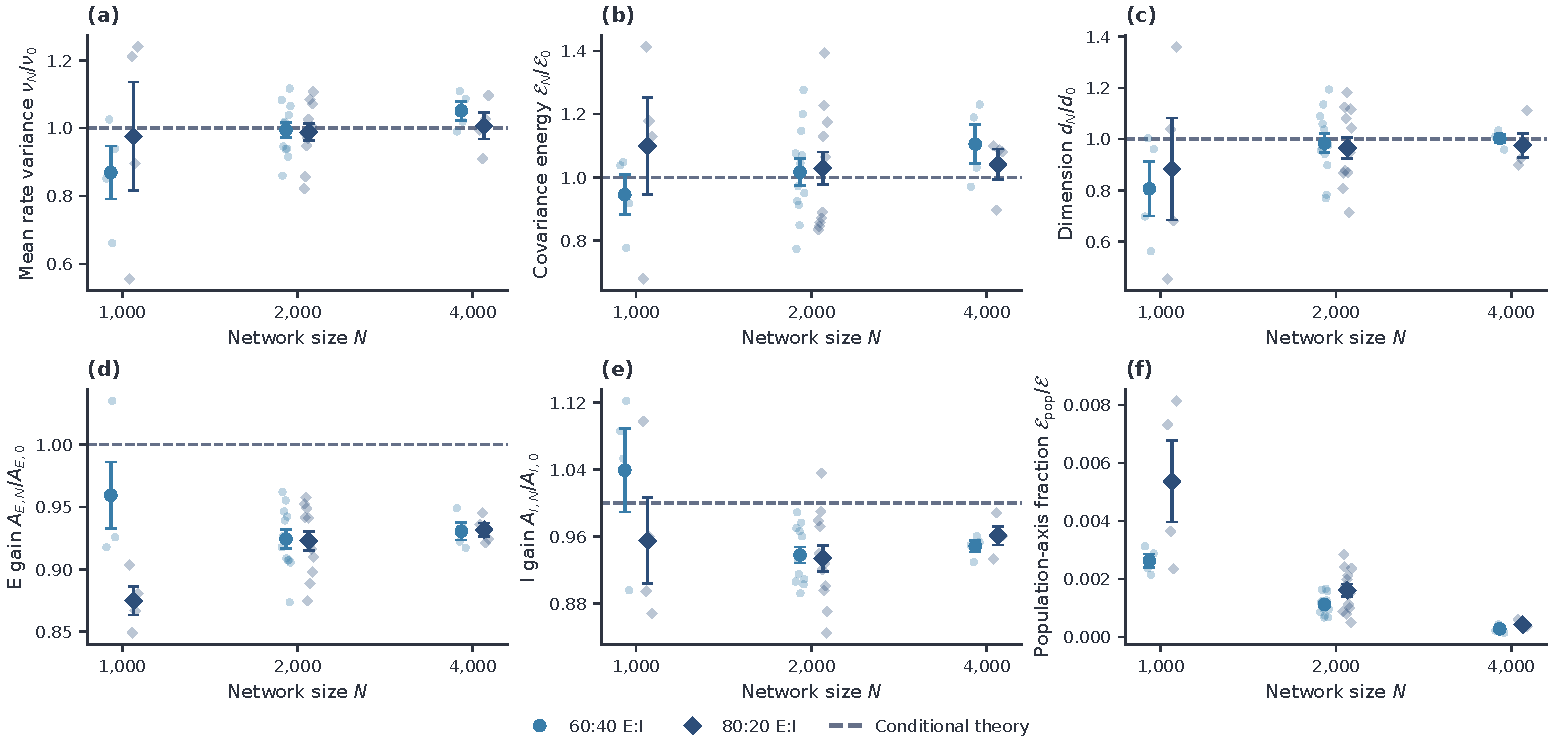
\includegraphics[width=\linewidth]{composition_validation.pdf}
\caption{\textbf{Ingredient checks accompany the PR comparison.}
Original 40-network composition and size series. Panels a--c show the original
moment and dimension comparisons for context. Panels d,e compare squared
time-averaged local slopes $A_a$ with their parameter-only values;
instantaneous squared slopes are a different observable. Panel f shows the
fraction of covariance energy involving a population-uniform direction,
including mixed uniform--transverse sectors. Points are networks and group
means with network standard errors. These checks distinguish local-law
errors from direct population-axis energy, without turning measured local
statistics into a parameter-only correction.}
\label{fig:ingredients}
\end{figure}

\FloatBarrier
\section{Historical unequal-lag population comparison}
\label{app:historical_lags}

The original handoff also tests the stronger two-lag prediction
\[
 \psi_{ab}(\tau_1,\tau_2)
 =N\mathbb E[C_{ij}(\tau_1)C_{ij}(\tau_2)
              \mid i\in a,j\in b,i\ne j]
\]
in the nonuniform 80:20 reference network. The historical cohort contains
seeds 77, 88, and 99 at $N=1000$, and seeds 77 and 88 at $N=2000$.
The recordings are 6000 and 8000 leak times, respectively, after 1000
burn-in times, with midpoint step $0.05$ and storage interval $0.25$.
Each map uses 12000 distinct sampled pairs per class and lags from $-24$
to $24$ in steps of one leak time. Within-class sampling restores both pair
orientations.

This historical estimator multiplies covariance estimates from separately
centered temporal blocks. There are eight blocks per recording; selected
block pairs have at least one empty block between them. The mean-difference
repair used by the fresh zero-lag campaign has not been applied to these
archived maps. Changing from eight to four centered blocks in the
$N=2000$, seed77 diagnostic changes the maps by about 6\%, so this comparison
must remain distinct from the current estimator validation.

At $N=2000$, relative Frobenius map errors are 9.3\%, 15.3\%, and 14.7\%
for E--E, E--I, and I--I, while flattened map correlations are 0.998, 0.995,
and 0.995. The dominant ridge and equal-lag decay are reproduced, but
negative unequal-lag lobes remain unexplained. High map correlation therefore
supports the broad temporal pattern, without establishing exact amplitudes
or tails. These historical networks do not increase the replication count
of the fresh staged campaign.

\begin{figure}[p]
\centering
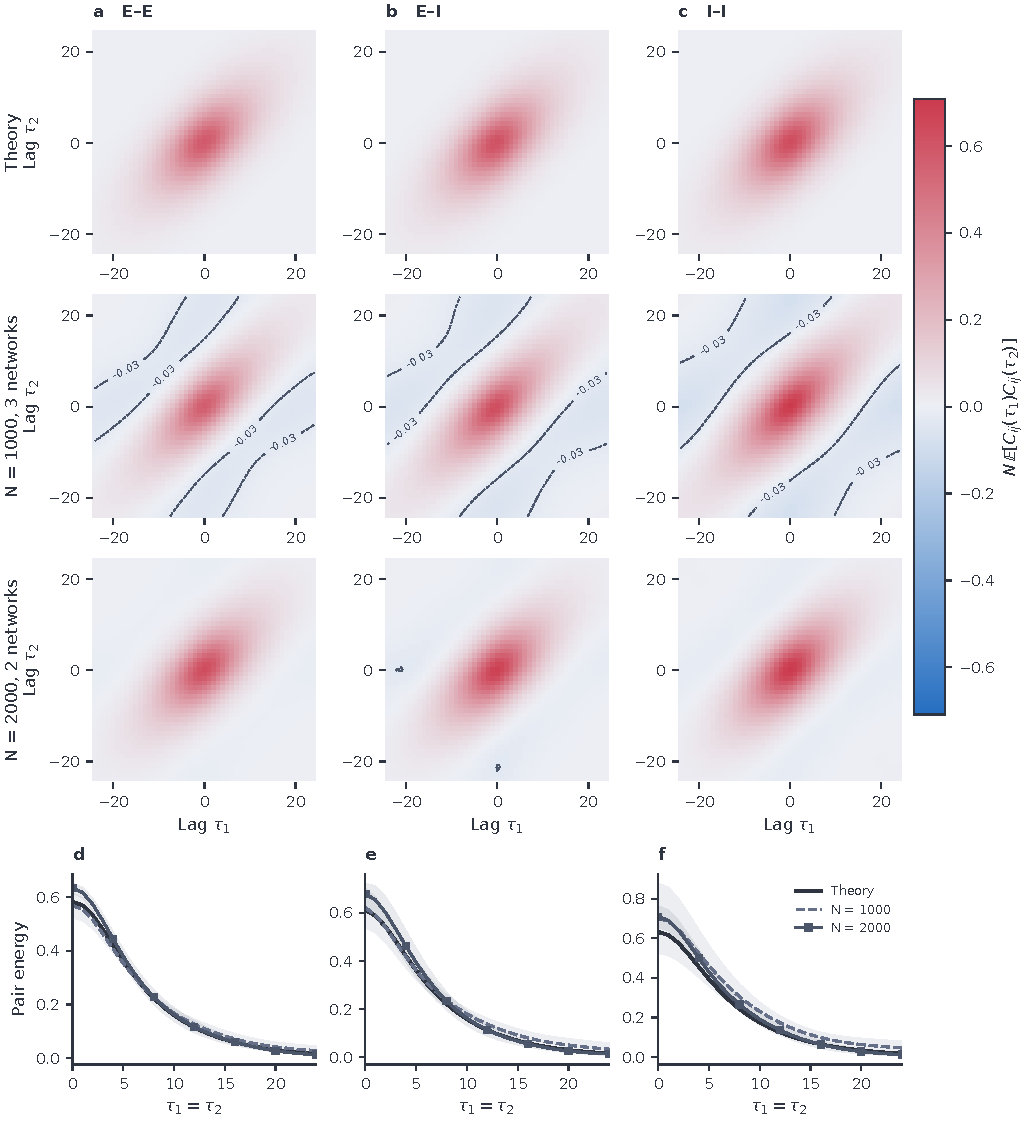
\includegraphics[width=.93\linewidth]{historical_lag_validation_nord.pdf}
\caption{\textbf{Historical evidence for population-resolved temporal structure.}
Lag maps from the original handoff, displayed with the paper's color scale.
Columns are E--E, E--I,
and I--I. The first row is parameter-only theory; the next rows are the mean
of three $N=1000$ and two $N=2000$ networks described in the text. Heatmaps
share one absolute color scale; dashed contours mark negative values.
The bottom row shows equal-lag slices, with sample standard-deviation bands
across networks, not across sampled pairs. No gain, amplitude, or timescale
is fitted to cross-neuron data. The historical separately centered estimator
and unresolved negative lobes restrict this evidence to the stated comparison.}
\label{fig:historical_lags}
\end{figure}

\FloatBarrier
\bibliographystyle{unsrtnat}
\bibliography{references}
\end{document}
